\documentclass{article}
\usepackage{graphicx} % Required for inserting images
\usepackage[utf8]{inputenc} % Per caratteri accentati
\usepackage[T1]{fontenc}    % Per una corretta codifica dei font
\usepackage[italian]{babel} % Per sillabazione in italiano
\usepackage{float}

\title{Architettura degli elaboratori}
\author{}
\date{}



\begin{document}
\maketitle


\paragraph{Indroduzione, NAND}



É la porta logica che sta alla base dei calcolatori, essa funziona attraverso due entrate (due fili), che attraverso la tabella di veritá NAND (Tabella \ref{tabella_nand} portano ad un output.


\begin{figure} [h!]
    \centering
    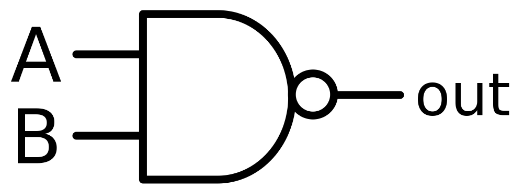
\includegraphics[width=0.25\linewidth]{nand foto.png}
    \caption{Simbolo della porta logica NAND}
    \label{fignandlogo}
\end{figure}



La logica che sta dietro all'output segue il nome NAND ovvero \textbf{"not"} e \textbf{"and"}: cosiderando 1 come vero e 0 come falso se volessimo descrivere a parole il processo sarebbe "la negazione dell'risultato dell'operazione di and logico". Per esempio consierando la prima riga della Tabella \ref{tabella_nand}: falso e falso risultano in falso che negato diventa vero, quindi 1.

\begin{table}[h!]
\begin{center} 
    \begin{tabular}{|c|c|c|} 
        \hline
        A & B & OUTPUT\\
        \hline
        0 & 0 & 1\\
        0 & 1 & 1\\
        1 & 0 & 1\\
        1 & 1 & 0\\
        \hline 
    \end{tabular}
    \caption{Tabella di veritá NAND}
    \label{tabella_nand}
\end{center} 
\end{table}

Per quanto riguarda la realizzazione pratica si tratta di un circuito abbastanza semplice composto da due transistor (i due input), una resistenza e un filo di output (Fig. \ref{fig_nand}).

\begin{figure} [H]
\centering 
    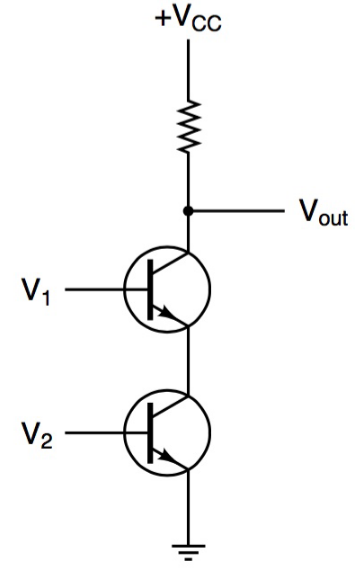
\includegraphics[scale=0.25]{Circuito nand}
    \caption{Circuito NAND}
    \label{fig_nand}
\end{figure}

Per controllare a livello fisico quale sia l'output del circuito si misura il voltaggio tra la resistenza e il primo transistor attraverso il filo di output. Nozione importante é quella del comportamento del transistor: se ha un'alta tensione (logicamente 1) si comporta come un conduttore ideale, mentre se non ha tensione (logicamente 0) si comporta come una resistenza infinita. Dunque, quando almeno uno dei due resistori non ha tensione la corrente e quindi il potenziale passano nel filo di output, mentre se hanno tensione entrambi la corrente passa nel conduttore ideale.


La NAND viene detta universale perché attraverso solo essa si possono costruire tutte le tipologie di porte logiche e attraverso milioni di esse anche calcolatori che eseguono programmi.


\section{Storia degli elaboratori}
Essa é necessaria per capire le scelte di progettazione dei moderni calcolatori andandone ad analizzare lo sviluppo. Il primo oggetto considerabile come calcolatore é la \textbf{Pascalina} ideata nel 1642 che peró era una semplice calcolatrice meccanica, circa un decennio dopo Leibnez ne ideó un'evoluzione capace di eseguire anche le moltiplicazioni e le divisioni. Il primo oggetto che si puó considerare un vero e proprio precursore dei calcolatoi moderni é l'\textbf{Analytic Engine}: esso era composto da 3 parti principali:
\begin{itemize}
    \item \textbf{Mulino}: addetto alla parte computazionale
    \item \textbf{Magazzaino}: la memoria
    \item \textbf{Input/Output}: forniti attraverso le schede perforate
\end{itemize}
La prima macchina che peró utilizzava circuiti elettrici fu \textbf{Zi}, ideata nel 1936, un calcolatore basato sull'utilizzo di relé che diede il via allo sviluppo degli anni successivi: grazie ai finanziamenti della Gran Bretagna per il secondo conflitto mondiale, nel 1945 venne costruito \textbf{Colossus} famoso per essere il calcolatore che riusciva a decifrare i codici nazisti. Per quanto riguarda la parte tecnologica i relé vennero sostituiti da delle valvole, nonostante questo tipo di tecnologia venne tenuta secretata per diverso tempo nel 1946 venne costruito \textbf{EINAC} un calcolatore che univa la tecnologia dei relé a quella delle valvole ma che aveva anche bisogno dello spostamento fisico di cavi.

Una grande rivoluzione avvenne nel 1952 quando \textbf{Von Neumann} ideó \textbf{IAS}, la rivoluzione non stava tanto nella tecnologia usata dal calcolatore ma quanto nella logica che stava dietro all'architettura di esso, la quale influenzerá quella di tutti i modelli successivi fino ai nostri giorni. La parte piú interessante riguarda l'architettura del processore: l'\textbf{unitá di controllo} regola l'esecuzione dei programmi da parte dell'\textbf{unità aritmetico-logica} la quale lavora sui dati contenuti all'interno dei \textbf{registri}, diversi dalla memoria (Fig. \ref{mrvon}).

\begin{figure}[H]
    \centering
    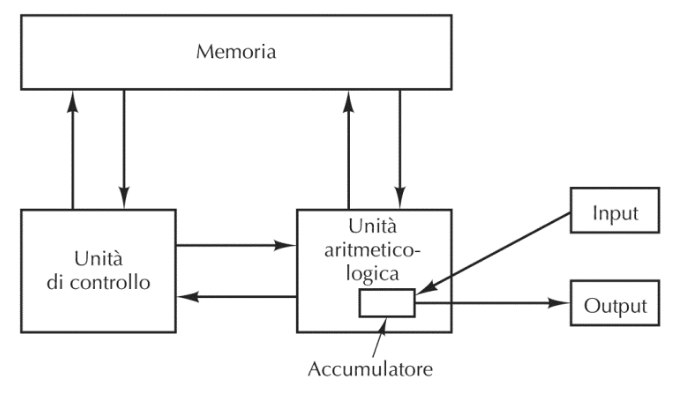
\includegraphics[width=0.75\linewidth]{arcvon.png}
    \caption{Architettura di Von Neumann}
    \label{mrvon}
\end{figure}

Nel 1961 si ha un'evoluzione per quanto riguarda la parte commerciale degli elaboratori, se fino ad ora essi erano pezzi unici creati da governi o aziende super-specializzate con \textbf{PDP-1} ora anche le accademie potevano dotarsi di un proprio elaboratore dotato di un'interfaccia grafica e non piú basato su relé o valvole ma su piú moderni transistor. Pochi anni dopo ci fu un ulteriore rivoluzione, questa volta per quanto riguarda la parte piú attinente all'esecuzione dei programmi, infatti il \textbf{CDC 6600} supportava il parallesimo: diverse unitá del calcolatore potevano gestire diverse operazioni svolte peró nello stesso momento. Nel 1964 l'IBM introdusse la prima famiglia di calcolatori con l'\textbf{IBM 360}, per famiglia si intendono diversi modelli che differiscono in base alle prestazioni ma anche per prezzo commerciale. A livello tecnico due furono le maggiori novitá:
\begin{itemize}
    \item \textbf{Multiprogrammazione}: possibilitá di eseguire in contemporanea piú di un programma.
    \item \textbf{Emulazine}: retrocompatibilitá del software giá scritto.
\end{itemize}

Nel 1980 si ha un'importante innovazione tecnologica che introduce i calcolatori \textbf{VLSI} (Very Large Scale Integration) cioé calcolatori con un elevatissimo numero di transistor nei chip, lo sviluppo di questa tecnologia segue la \textbf{Legge di Moore} ovvero lo sviluppo, inteso come quantitá di transistor nello stesso spazio, é aumentato del 60\% ca. ogni anno. L'anno successivo esce \textbf{IBM 5150}, il primo personal computer e ne vengono pubblicati schemi e dettagli dell’architettura per semplificare il progetto di schede di espansione.
Anche il sistema operativo MS-DOS (Microsoft Disk Operating System) venne sviluppato nello stesso anno ma non venne realizzato da IBM bensí dalla Microsoft Corporation (allora piccolissima software house).

\section{Unità di misura e prefissi per gli ordini di grandezza}

\begin{figure} [H]
    \centering
    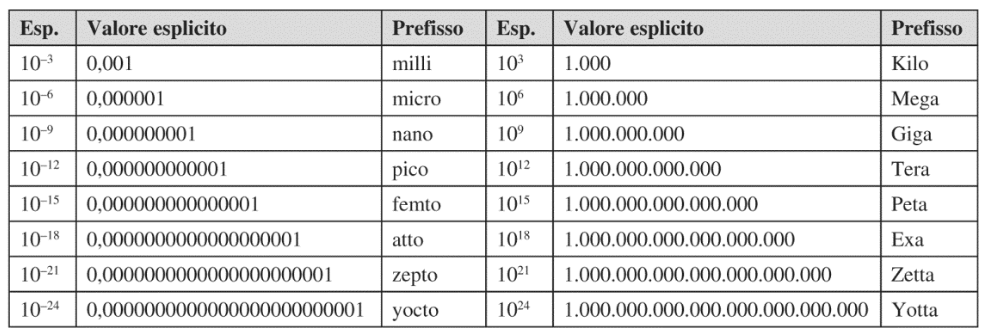
\includegraphics[width=1.14\linewidth]{tab.png}
    \caption{Principali prefissi}
    \label{pref}
\end{figure}

\begin{itemize}
    \item \textbf{MIPS}: milioni di operazioni per secondo.
    \item \textbf{GFLOPS}: miliardi di operazioni floating-point per secondo.
\end{itemize}


\section{Organizzazione degli elaboratori}

\begin{figure} [H]
    \centering
    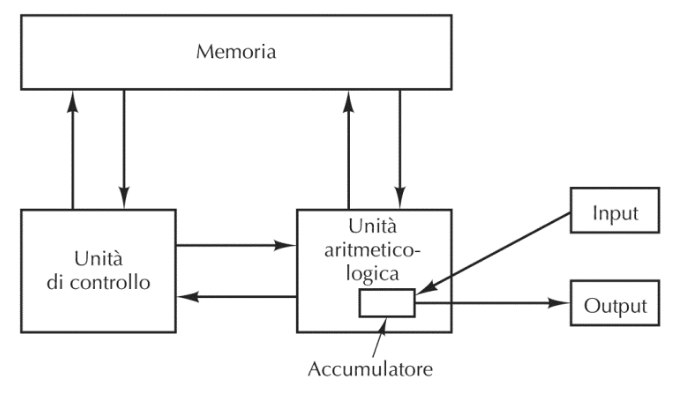
\includegraphics[width=0.5\linewidth]{arcvon.png}
    \caption{Architettura di Von Neumann}
    \label{ripevon}
\end{figure}

 Di seguito una descrizione piú esaustiva della Fig. \ref{ripevon}.

 \paragraph{Frecce} sono chiamate bus di trasporto e consentono di scambiare dati, a livello pratico sono un insieme di fili dello stesso numero dei bit che usa il processore ad ogni calcolo.
 Si possono dividere in due categorie princilpali:
 \begin{itemize}
     \item \textbf{(sotto) bus dati}
     \item \textbf{(sotto) bus indirizzi}
 \end{itemize}

 
\begin{figure} [h!]
    \centering
    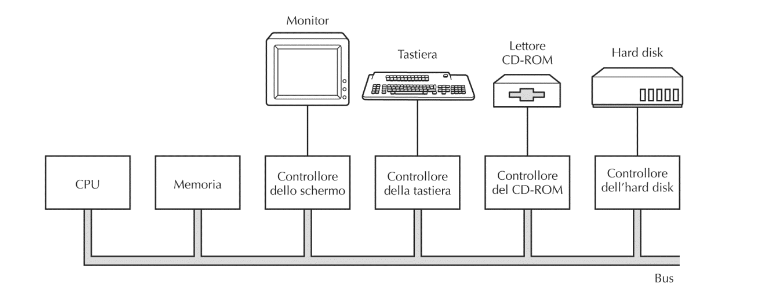
\includegraphics[width=0.7\linewidth]{esempio bus.png}
    \caption{Esempio di bus di trasporto}
    \label{bus}
\end{figure}

\paragraph{Controllori} essi (non mostrati in Fig \ref{ripevon}) operano da traduttori per i dispositivi in input/output peró sono \textbf{unici} per il singolo dispositivo in questione (es. un hard disk).

\paragraph{Memoria RAM} la si può sia leggere che scrivere, puó contenere sia dati che programmi e a livello fisico è fatta da svariate locazioni di memoria indicate con indirizzi. Gli indirizzi di queste locazioni solitamente viaggiano solo dal processore alla memoria, sono quindi monodirezionali.


\paragraph{CPU (Central Processing Unit)} é composta da diverse parti:
\begin{itemize}
    \item \textbf{ALU}: esegue tutte le operazioni logico-aritmetiche che sono "ordinate" dalla contol unit.
    \item \textbf{control unit}: legge il codice macchina, ne interpreta le istruzioni e delega il lavoro alle parti dedicate ad ogni specifica operazione.
    \item \textbf{registri}: singole locazioni di memoria che contengono i dati prima o dopo essere stati processati dalla ALU e che sono interni al processore in modo tale da avere uno scambio piú rapido. Essi si possono dividere in diversi tripi in base alla loro funzione:
        \begin{itemize}
            \item \textbf{Program Counter}: contiene il numero dell'istruzione che deve essere eseguita.
            \item \textbf{Instruction Register}: dove viene copiata l'informazione scritta nella cella puntata dal Program Counter, ovvero l'istruzione da eseguire
            \item \textbf{Memory Address Register}: dove viene registrato il numero di indirizzo della cella di memoria dove si deve andare a prendere l'input, come tappa intermedia per semplificare il circuito a livelo fisico
            \item \textbf{Memory Data Register}: registra l'informazione prelevata dal bus dati dalla casella puntata dalla MAR, anche in questo caso come tappa intermedia.
            \item \textbf{Program Status Word}: insieme di bit che funzionano da flag per tenere traccia di eventi rilevanti nell'esecuzione come errori o particolari risultati.

        \end{itemize}
    
\end{itemize}
Schematicamente i passaggi possono essere visti nel seguente modo:
\begin{center}
     PC $\rightarrow$ MAR $\rightarrow$ Cella $\rightarrow$ MDR $\rightarrow$ IR
\end{center}


\paragraph{Quindi, come funziona l'esecuzione di un programma?} 


\begin{enumerate}
    \item il contenuto della cella di memoria puntata da PC viene copiato in MAR
    \item il contenuto nella memoria di indirizzo puntato da MAR viene copiato in MDR
    \item il contenuto di MDR viene copiato su IR e decodificato dalla control unit
    \item ALU esegue le operazioni logoico aritmetiche
    \item se ci sono operandi da prelevare in memoria si allocano nei registri (con MAR e MDR)
    \item finite le operazioni il risultato è messo sul registro destinazione, se bisogna scrivere i dati in memoria attraverso MAR e MDR si attiva la linea di scrittura che, ovviamente, segue le istruzioni della CU.
    \item Si torna ad 1 con PC aggiornato
\end{enumerate}

\begin{center}
    \textbf{IMPORTANTE}: \textit{tutto questo processo è governato dalla Contorol Unit}
\end{center}

Sempre parlando di come viene eseguito un programma, si possono definire diverse fasi dello svolgimento:
\begin{itemize}
    \item \textbf{Fetch dell'istruzione}: prelievo dell'istruzione dalla memoria e la decodifica di essa. [passi 1-2]
    \item \textbf{Fetch dei parametri}: prelievo del parametro dalla memoria 
    \item \textbf{Decode}: identificazione dell'operazione da eseguire [passo 3]
    \item \textbf{Execute}: esecuzione dell'istruzione [4-5-6]
\end{itemize}


\paragraph{Multiplexer} é un circuito elettronico digitale la cui grandezza d'uscita è uguale a quella di entrata per quanto riguarda il volume di informazioni, il suo compito é trasmettere uno solo un dato nonostante ne prenda in input due: questa operazione é possibile grazie ad un selettore il cui valore decide l'output. Il multiplexer é collegato sia prima che dopo l'ALU.

\begin{figure} [h!]
    \centering
    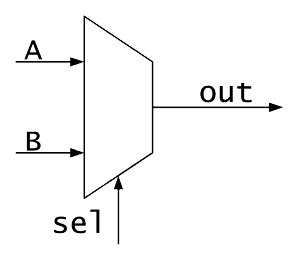
\includegraphics[width=0.3\linewidth]{Multiplexer.png}
    \caption{Simbolo multiplex}
    \label{multiplex}
\end{figure}

\paragraph{JZ (jumping zero)} se il PSW rileva che il risultato dell'istruzione precedente è 0, o altro valore arbitrario, salta ad una data istruzione tramite un multiplexer, anche questo processo é regolato tramite la Control Unit.

\paragraph{Control Unit} essa è un oggetto abbastanza complicato, per realizzarla si può costruire o un singolo e grosso circuito che prevede ogni singola istruzione oppure si puó usare un assembler più semplice e vedere la CU come un ulteriore processore. Quest'ultimo approccio non è più semplice, però ha dei vantaggi tipo poter modificare le istruzioni perché sono nella memoria e non in un circuito statico, inoltre si posssono anche eseguire diverse operazioni sugli stessi circuiti.


\paragraph{Clock} é il componente che dá il tempo a tutte le azioni: all'inizio di un ciclo di clock i componenti iniziano a calcolare con i dati che hanno in quel momento, quando è 0 o simili si "fanno i calcoli". In definitiva piú alta é la frequenza del clock piú operazioni al secondo la CPU riesce a fare, questa frequenza é il risultato di tutti i fattori e i componenti che compongono la CPU. Fisicamente è un cavo con un segnale dato dalla vibrazione di dei cristalli che crea dei picchi e dei minimi.

\begin{figure} [H]
    \centering
    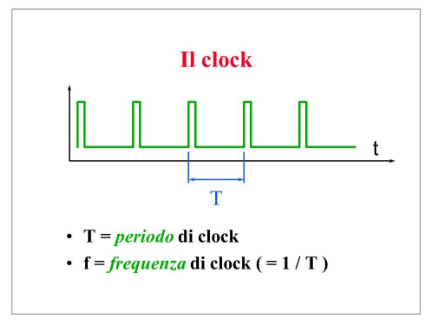
\includegraphics[width=0.5\linewidth]{clock.png}
    \caption{Valori clock nel tempo}
    \label{clockr}
\end{figure}





\textit{Come fare quindi ad aumentare le prestazioni della CPU senza overclocking?}

La risposta a qusta domanda é il \textbf{parallelismo} ovvero fare tante operazioni in contemporanea, concretamente ci possono essere diverse soluzioni:
\begin{itemize}
    \item \textbf{Pipeling}: sfrutta l'idea della catena di montaggio, si divide la CPU in vari pezzettini e solo una parte dell'esecuzione (tipo accede alla memoria oppure la decodifica) viene eseguita dal singolo pezzettino in modo che la prima istruzione ci mette un po' più tempo rispetto alle successive, ma appena tutte e 5 lavorano a regime ad ogni ciclo di clock si finisce un'istruzione. Così facendo si va nettamente più veloce senza dover comprare altre ALU perché ne basta solo 1 ma ci possono essere dei problemi in alcuni casi, per esepio con JZ.

    \begin{figure} [h!]
        \centering
        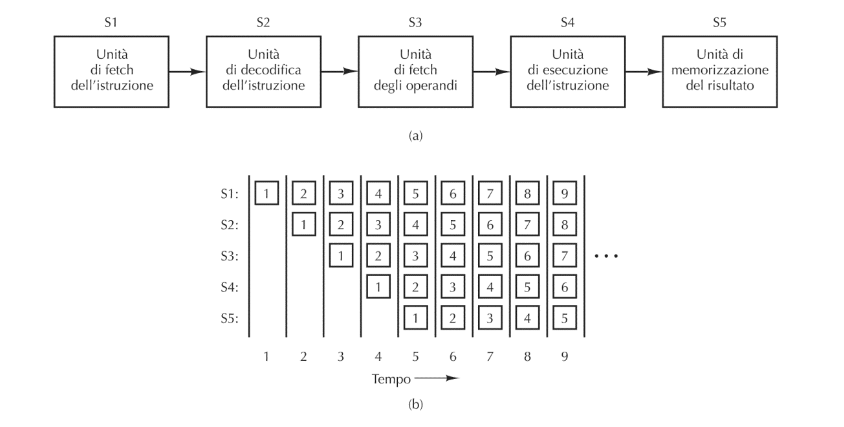
\includegraphics[width=0.7\linewidth]{Pipeling.png}
        \caption{Schema del pipeling}
        \label{fig:}
    \end{figure}
    
    \item \textbf{Multicore} (core = processore): la CPU ha diversi processori collegati tra di loro con una cache condivisa. In questo caso ci sono proprio diverse ALU, a livello pratico di solito nelle CPU multicore ci sono più core di quelli usabili per possibili errori nella
    produzione.
    \item \textbf{SIMD} (Single Istruction-Stream, Multiple Data-Stream) tante piccole ALU e registri (connessi ad esse) che processano le informazioni seguendo però la stessa CU in modo vettoriale, quindi sono molto veloci a fare la stessa operazione su elementi diversi. Le schede grafiche, per esempio, sono costruite secondo questa filosfia utile nel mining di bitcoin oppure nelle reti neurali e machine learning.

\begin{figure} [h!]
    \centering
    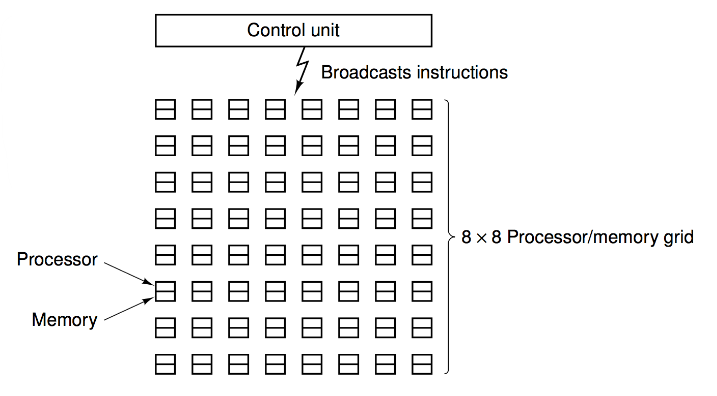
\includegraphics[width=0.75\linewidth]{Simd.png}
    \caption{Esempio visivo di un SIMD}
    \label{simd}
\end{figure}
    
    \item \textbf{Multiprocessori}: tanti processori con le singole memorie locali che però vengono collegati tutti a una memoria comune, le memorie locali sono necessarie per evitare che la velocità della memoria sia un collo di bottiglia.

\begin{figure} [h!]
    \centering
    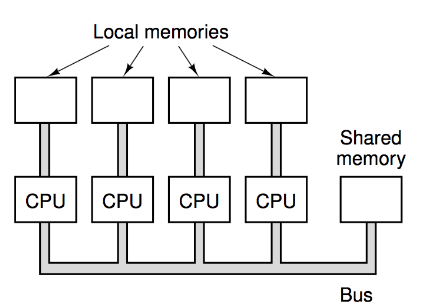
\includegraphics[width=0.5\linewidth]{Multiprocessori.png}
    \caption{Esempio di multiprocessori}
    \label{multiprocessori}
\end{figure}
    
    \item \textbf{Multicomputer}: parallelismo più estremo, sono le reti di computer.

\end{itemize}



\section{Le memorie}

\begin{figure} [H]
    \centering
    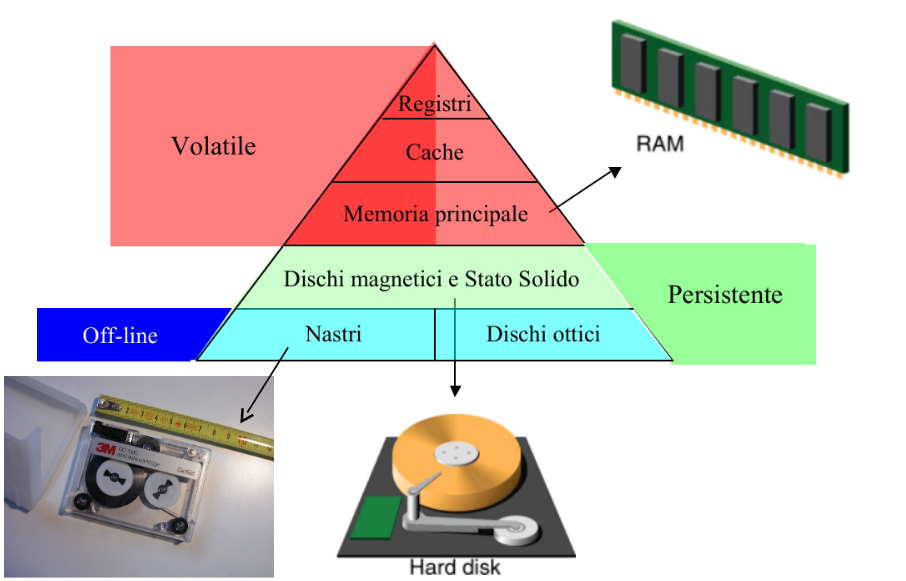
\includegraphics[width=0.85\linewidth]{memorie.png}
    \caption{Schema memorie, anche gerarchico}
    \label{mem}
\end{figure}

La terminologia non è sempre uniforme però tendenzialmente quando si parla di "memoria" si intende la RAM (Random Access Memory). La memoria, per una serie di motivi quali la distanza, la dimensione (infatti idealmente c'è un grande multiplexer  che estrae dati dalle varie celle di memoria) e altri motivi tecnologici è molto più lenta dei registri. D'altro canto la RAM rimane necessaria perché i registri possono contenere solo pochi dati, per queste motivazioni è stata inventata la \textbf{cache} ovvero una via di mezzo tra registri e ram: è più veloce della ram ma più lenta dei registri, più piccola della ram ma più grande dei registri. Essa contiene i dati che servono più spesso al processore al fine di accelerare l'accesso di memoria. Anche questa memoria però è volatile, quindi servono delle memorie permanenti tipo hard-disk (online rispetto al calcolatore) o nastri e dischi ottici (offline rispetto al calcolatore). C'è anche una gerarchia di memoria e cresce anche il prezzo per memoria dei singoli componenti.


Le memorie sono organizzate in celle ovvero sequenze di bit con uno specifico indirizzo, dagli anni '60 si usano i byte come standard 
Generalmente i blocchi sono sui 32/64 bit, tali blocchi di memoria vengono detti \textbf{"word"}; esistono 2 modi per memorizzare le word in celle di dimensione di 1 byte: in ordine crescente o decrescente. 

\begin{figure} [H]
    \centering
    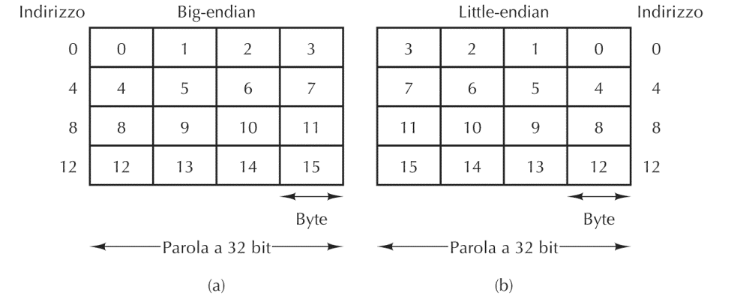
\includegraphics[width=1\linewidth]{word org.png}
    \caption{a. Memoria big endian, b. Memoria little endian}
    \label{word}
\end{figure}

\paragraph{Funzionamento cache}
La cache è a metà tra la CPU e la RAM ed è trasparente per la CPU perché intercetta la richiesta nel data bus e se ha le informazioni nella cella richiesta trasmette subito l'informazione, se no va nella memoria. Questo passaggio è utile perché i nostri programmi non accedono a caso nelle celle di memoria, infatti seguono il\textbf{ principio di località}: se si accede ad una locazione di memoria è molto probabile che nel futuro si accederà o alla stessa o ad allocazioni vicine (non è dimostrabile ma è molto probabile). Per cui la cache si ricorda cosa é già stato chiesto e conosce anche l'indirizzo delle celle vicine a quella a cui si é appena fatto l'accesso. A questo punto queste celle di memoria vengono salvate nella cache in modo da velocizzare tutti i processi, sempre peró a livello statistico.

\begin{figure} [h!]
    \centering
    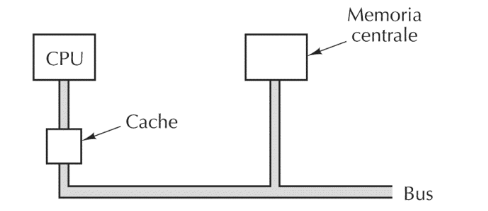
\includegraphics[width=0.75\linewidth]{cache.png}
    \caption{Schematizzazione della posizione della cache}
    \label{chace}
\end{figure}

Matematicamente: 

    c = tempo di accesso alla memoria cache
   
    m = tempo di accesso alla memoria centrale
    
    h = hit-ratio ovvero la frazione di domande a cui la cache può rispondere. 

    t = tempo medio di accesso
\begin{center}
    $t = c*h+(1-h)*(c+m)$
\end{center}
(il primo addendo analizza il caso in cui la cache abbia il dato necessario, il secndo quando invece non ha il dato), alla fine si otterrá
\begin{center}
    $t=c+(1-h)*m$ 
    
    il $\lim_{h\to1}$ sará appunto solo c (il caso in cui il dato é nella cahe)  
\end{center}
Ci sono due modi per aumentare h: o la cache è più grande oppure quando si scrivono i programmi si ottimizzano per la cache.

\paragraph{Hard-disk} dispositivo elettro-meccanico che serve a conservare le informazioni sotto forma magnetica, é composto da: 
\begin{itemize}
    \item \textbf{Testina magnetizzata}: legge/scrive lo stato di magnetizzazione della superficie
    \item \textbf{Traccia}: sequenza circolare di bit
    \item \textbf{Settore}: archi di circonferenza con una quantità fissata di bit.
\end{itemize}
\begin{figure}[h!]
    \centering
    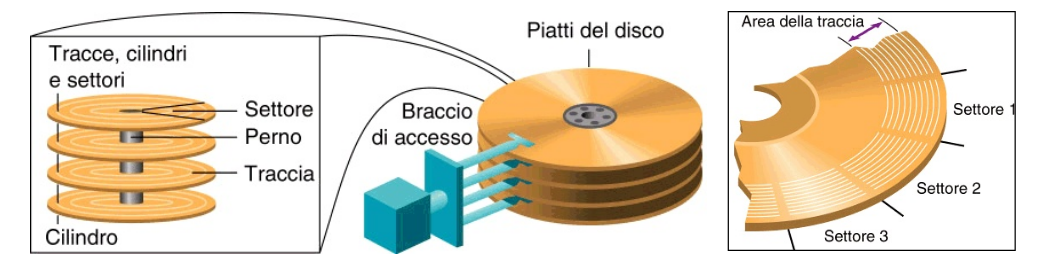
\includegraphics[width=1\linewidth]{HD.png}
    \caption{Schema di un Hard Disk}
    \label{HD}
\end{figure}
\paragraph{SSD} hanno la stessa funzione dell'Hard Disk ma sono un po' più moderni, inoltre sono puramente elettronici quindi non sono più definibili come memorie solide e per questo consumano meno energia; dal punto di vista di prestazioni hanno meno capacità ma prestazioni più veloci.
La discrepanza però tra velocità della CPU e degli HD o SSD si sta sempre di più allargando quindi se ne usano, generalmente, più unitá in parallelo. Inoltre la probabilità di perdere dati non è nulla quindi serve \textbf{ridondanza}, essa rende un dato più voluminoso ma si sposa bene con il parallelismo per stare dietro alla velocitá della CPU.
\paragraph{CD} usano un principio ottico che legge la riflessione da parte del disco, in base alle rifrazioni si ottengono 0 e 1 che codificano informazioni.
\section{Altre periferiche}
\paragraph{Monitor} richiede una specifica scheda video che contiene un proprio processore detto GPU (Graphical Processing Unit) perché ogni singolo pixel deve essere computato visto che il colore é generalmente codificato da diversi bit. Per questa ragione sono degli oggetti molto complicati.

\paragraph{Interrupt} Le altre periferiche sono collegate tra di loro e alla CPU attraverso i bus e un dispositivo detto "controller", alcuni di questi controller accedono direttamente alla memoria con una tecnica detta \textbf{DMA} (direct memory access). La tecnica consiste nel gesire autonomamente il processo di passaggio di file da una periferica all'altra (per esempio le memorie) e alla fine viene mandato un segnale di "\textbf{interrupt}" alla CPU, facendo questo si libera la CPU dal lavoro di quel tipo di operazione. 
L'interrupt peró viene anche usato da altre periferiche sempre verso la CPU, per esempio dalla tastiera: per evitare che la CPU stia sempre ad aspettarsi un input essa manda un "interrupt" ad ogni input mandato in modo tale che la CPU iterrompa le altre operazioni per ricevere l'input della tastiera.

\section{Porte logiche e circuiti combinatori}  

\begin{figure} [H]
    \centering
    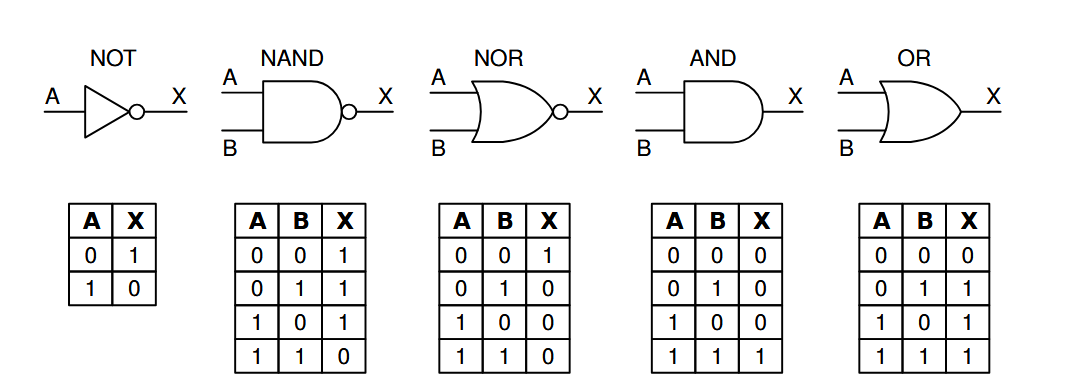
\includegraphics[width=1\linewidth]{porte logiche.png}
    \caption{Porte logiche}
    \label{porte logiche}
\end{figure}

Per farli esiste l'algebra di Boole che ci aiuta a per queste cose, ha tre operazioni:
\begin{itemize}
    \item \textbf{Addizioni}: 0+0=0, 0+1=1, 1+0=1, 1+1=0 (or)
    \item \textbf{Moltiplicazione}: 0*0=0, 0*1=0, 1*0=0, 1*1=1 (and)
    \item \textbf{Negazione}: $\bar{0}$=1, $\bar{1}$=0 (not)
\end{itemize}
Queste operazioni hanno anche delle proprietá tipo:
\begin{figure}[H]
    \centering
    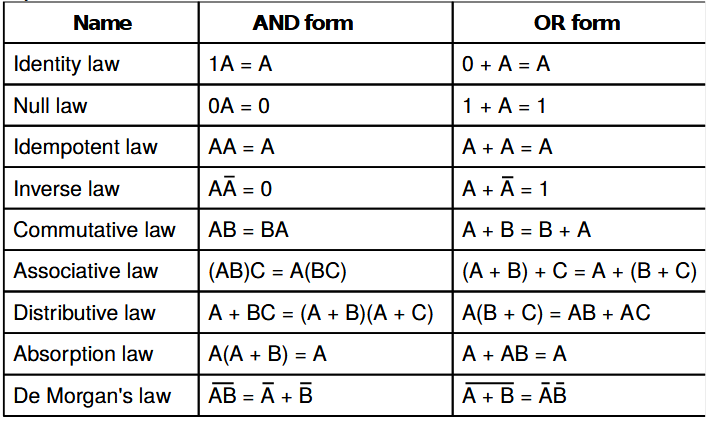
\includegraphics[width=0.85\linewidth]{proprietá logca bol.png}
    \caption{Proprietá delle operazioni algebriche Booleane}
    \label{prop}
\end{figure}


\paragraph{Le funzioni Booleane} associano alle variabili booleane input un valore logico in output, per comprendere e gestire meglio queste funzioni logiche si possono fare delle tabelle di verità. C'é una correlazione binaria tra il numero di righe e il numero di colonne. Infatti:
\begin{center}
    $righe = 2^{n. colonne}$
\end{center}

\textbf{Mintermini} utili per calcolare un'espressione che riporta gli stessi risultati della tabella. Per farla ad ogni riga si scrivono come $and$ tutte le variabili con annessa negazione/affermazione. Una volta finita questa operazione si crea un'espressione di $or$ con tutti gli $and$ che hanno un output $true$, (Fig. \ref{minter}).

\begin{figure} [H]
    \centering
    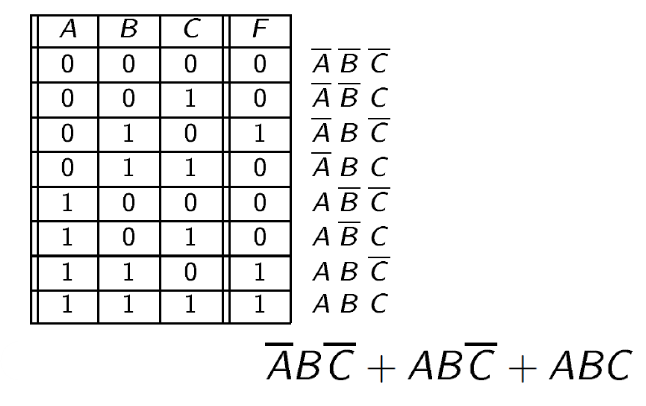
\includegraphics[width=0.65\linewidth]{MIntermini.png}
    \caption{Come i mintermini aiutano a trovare un espressione}
    \label{minter}
\end{figure}

\paragraph{Come implementare le funzioni booleane} si parte dalla NAND perché attraverso di essa si può fare qualsiasi circuito digitale (Fig. \ref{plNAND}). 

\begin{figure} [H]
    \centering
    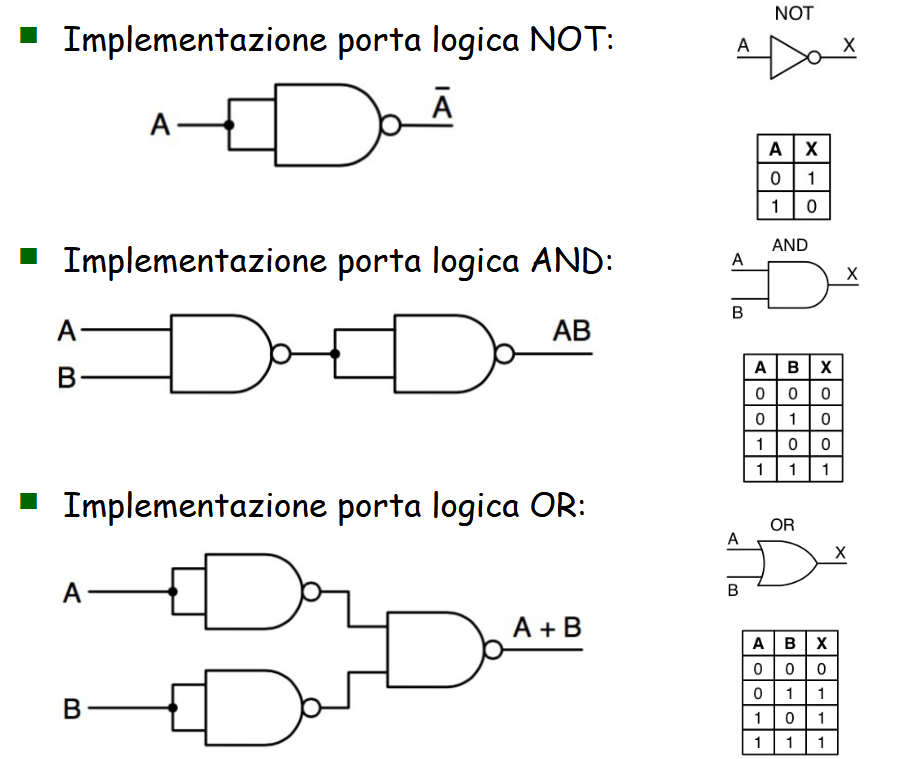
\includegraphics[width=0.75\linewidth]{Porte logiche nand.png}
    \caption{Esempio di come si possono implementare tutti i cancelli logici con la NAND}
    \label{plNAND}
\end{figure}

L'idea di usare le nand per tutti i circuiti digitali è puramente ideale, nella realtà dei fatti  ci sono implementazioni diverse.
In realtà esiste anche la Xor come porta universale, da 1 solo se uno dei due input è uno. 

\paragraph{PLA (Array Logici Programmabili)}
Sono circuiti universali precostruiti che data una quantità di input attraverso AND per tutti i possibili mintermini si collegano ad un grande OR finale. Attraverso la rottura di fusibili intermedi si può programmare il circuito per la data funzione che si vuole implementare (Fig.\ref{pla})

\begin{figure} [H]
    \centering
    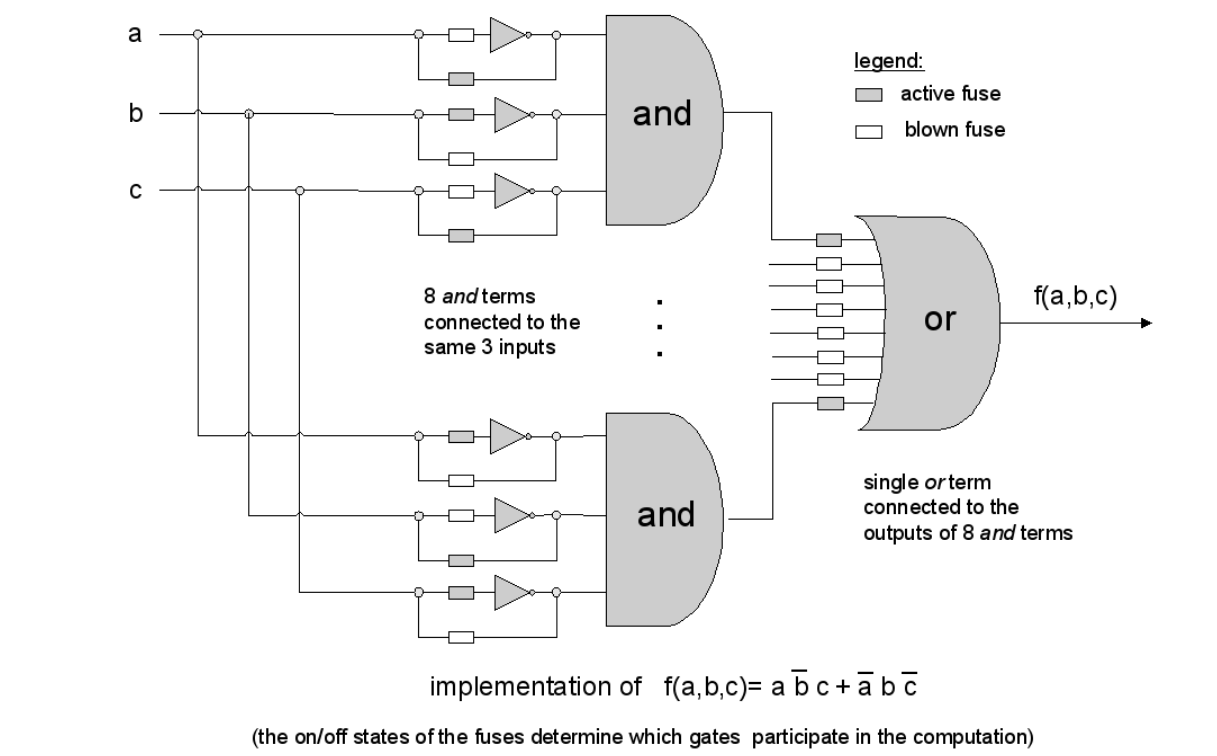
\includegraphics[width=1\linewidth]{PLA.png}
    \caption{Esempio di utilizzo di un PLA}
    \label{pla}
\end{figure}

\paragraph{Mappa di Karnaugh}
Modo utile e diverso dalle tabelle di verità che rende rende meccanico il capire come semplificare il circuito al massimo infatti il circuito combinatorio ottenuto si dice \textbf{minimale.}
Per fare la mappa di Karnaugh bisogna:
\begin{itemize}
    \item Creare una tabella bidimensionale con una cella per ogni possibile mintermine
    \item Far differire le celle adiecenti di solo una cifra, secondo il \textbf{codice Gray} (00 01 11 10).
    \item Completare la tabella con $1$ se la combinazione di input é $true$ o con $0$ se é $false$
\end{itemize}
\begin{figure} [H]
    \centering
    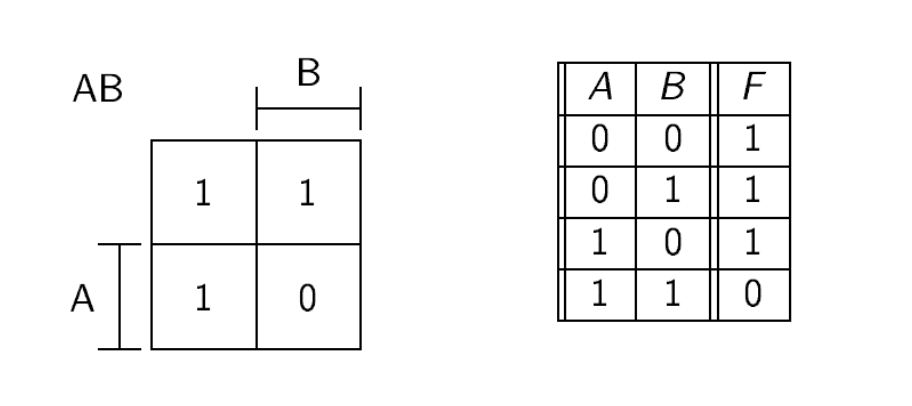
\includegraphics[width=0.75\linewidth]{mk 2.png}
    \caption{Esempio di mappa di Karnaugh con 2 variabili}
    \label{mk2}
\end{figure}

\begin{figure} [H]
    \centering
    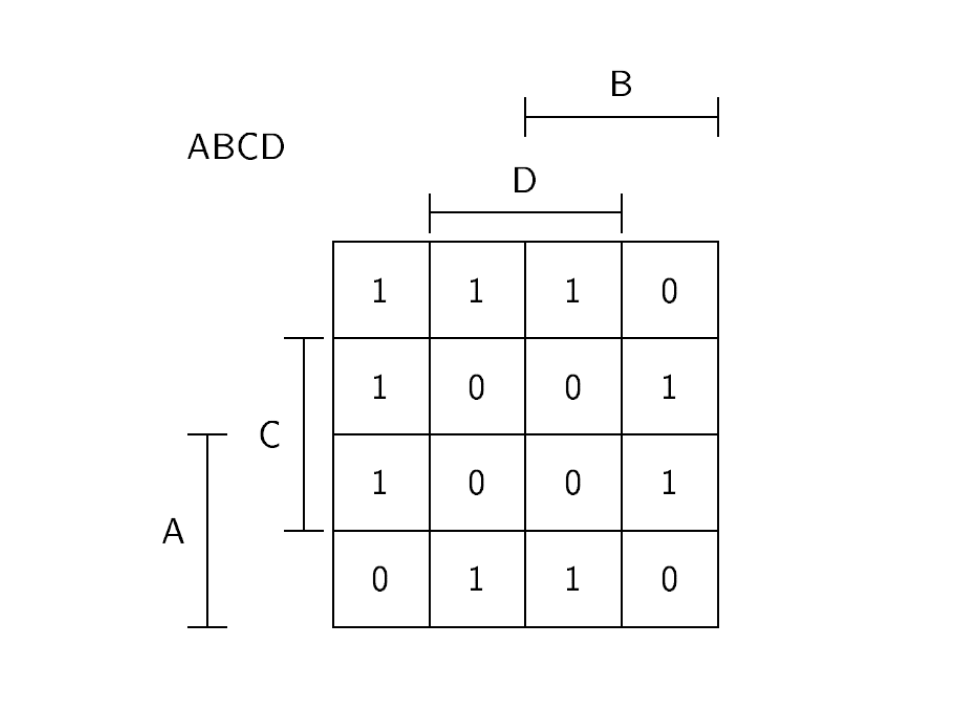
\includegraphics[width=0.75\linewidth]{mk4.png}
    \caption{Esempio di mappa di Karnaugh a 4 variabili}
    \label{mk4}
\end{figure}

A questo punto si identificano i rettangoli (anche quadrati) di celle che sono adiacenti e multipli di 2 per formare un \textbf{raggruppamento}. A questo punto i raggruupamenti si scrivono come prodotti booleani delle variabili che nello specifico raggrupamento non cambiano di valore. In altre parole si stanno eliminando le varibili che nel raggruppamento assumono entrambi i valori poiché questo implica che l'output non dipende da esse. Alla fine si fa un $OR$ tra tutti i prodotti ottenuti.

\begin{figure}[H]
    \centering
    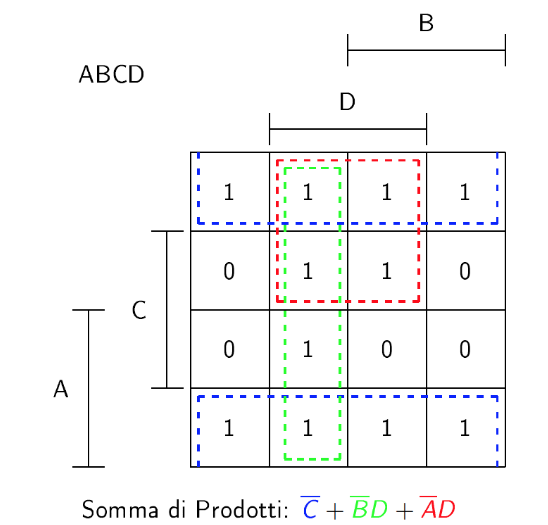
\includegraphics[width=0.75\linewidth]{es mk.png}
    \caption{Esempio di esercizio}
    \label{mkes}
\end{figure}


\textbf{NB.} il raggruppamento deve essere \textbf{minimale} nel senso che non si deve puntare a fare piú raggruppamenti possibili ma fare meno raggruppamenti possibili prendendo tutti gli 1 possibili. Inoltre ci sono tipi di raggruppamenti particolari (Fig. \ref{mkes2}).

\begin{figure} [H]
    \centering
    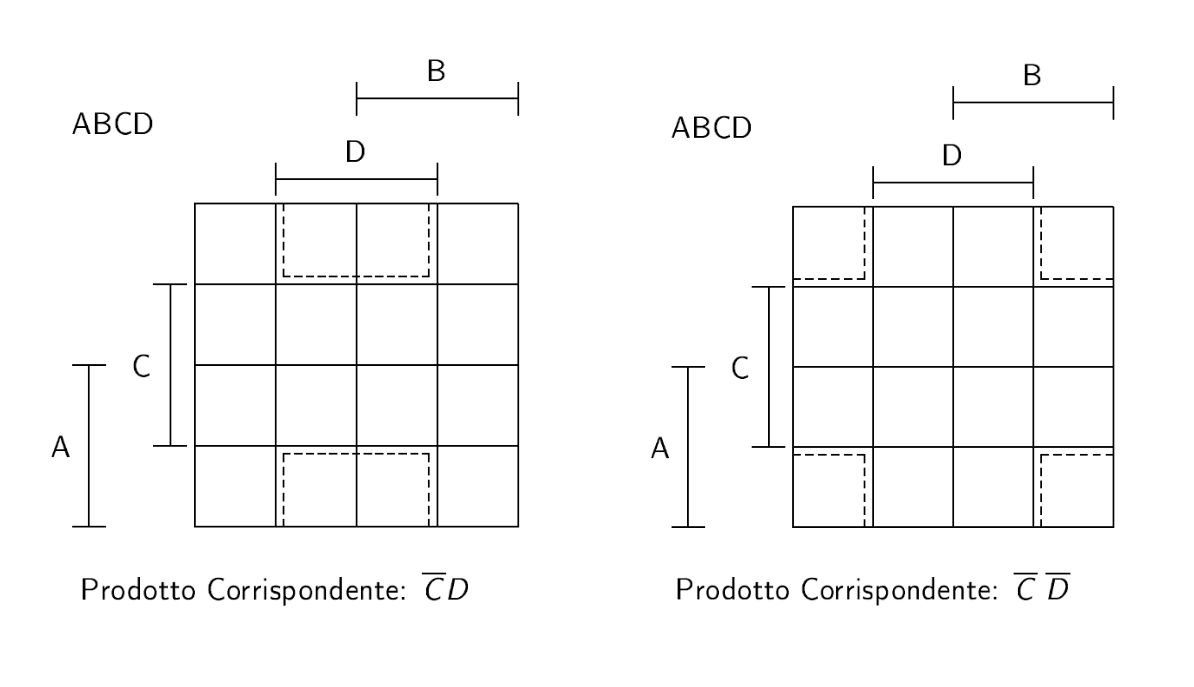
\includegraphics[width=0.95\linewidth]{esmk2.png}
    \caption{Esempi di particolari raggruppamenti}
    \label{mkes2}
\end{figure}


\section{Circuiti sequenziali}

\begin{figure}[H]
    \centering
    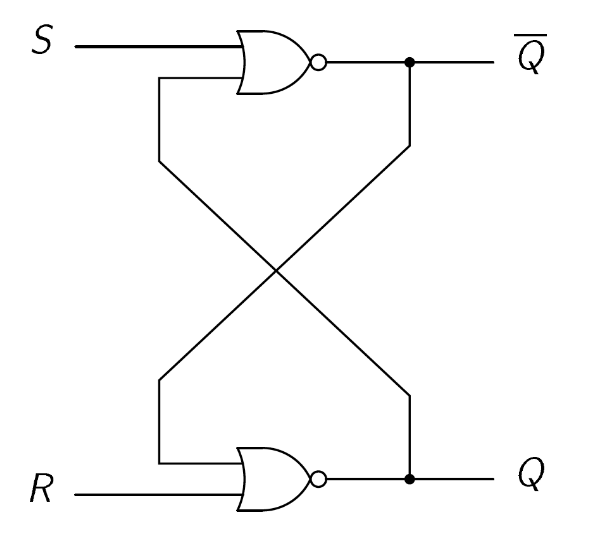
\includegraphics[width=0.5\linewidth]{cirseq.png}
    \caption{Esempio di circuito sequenziale: Latch SR}
    \label{circseq}
\end{figure}
Sono necessari perché i circuiti combinatori non si ricordano dati passati, quindi per fare memorie, registri, ecc... servono questo tipo di circuiti. La differenza principale con i circuiti combinatori è che gli output non dipendono solo dagli input ma anche dagli output passati in modo tale da poter memorizzare un certo valore. Nel caso dell'esempio in figura mettendo S = 1 e R  = 0, partendo da S e sfruttando la tabella di verità del nor so che $\bar{Q} = 0$ e $Q = 1$. Essendo il circuito simmetrico, finchè c'è un 1 la tabella dei verità è facile da fare, nel caso in cui si scelga 0 e 0 bisogna andare per tentativi e non si conosce precisamente l'output:

\begin{figure}[H]
    \centering
    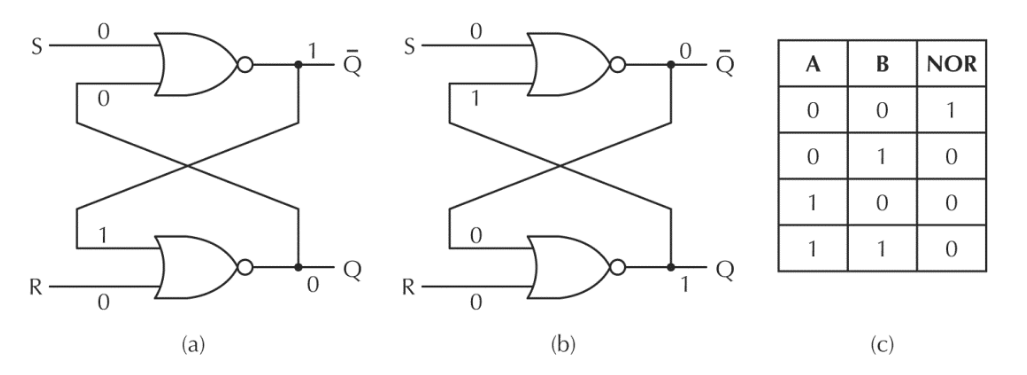
\includegraphics[width=0.95\linewidth]{Latchsrio.png}
    \caption{(a) Latch di tipo NOR nello stato 0. (b) Latch di stato NOR nello stato 1. (c) Tabbele di veritá del NOR}
    \label{latcio}
\end{figure}
Con questo tipo di circuito peró si presta sempre attenzione a non impostare mai 1 come input sia in S che R in modo tale che i due output siano sempre diversi, piú in particolare si vuole che l'ultimo seganle sia quello che si vuole memorizzare e che sia Q = 1 se é S l'ultimo segnale, se no Q = 0 quando R é l'ultimo segnale (per ultimo segnale si intende quale dei due é posto a 1).

\textbf{Clock}:  si collega il latch SR con un clock in modo che quando il clock è 0 si ricorda gli ingressi, mentre quando è 1 "sovrascrive" creando il Latch SR temporizzato che cambia il proprio stato solo in particolari momenti. (Fig.\ref{Ltemp})

\paragraph{Latch D temporizzato} D sta per dato e D viene collegato a S e negato in R, è interessante perché trattiene il segnale più a lungo rispetto ai precedenti tipi di latch. (Fig.\ref{ldtemp})

\paragraph{Latch DDF} Si prende il clock, si sdoppia e in un caso si nega poi entrambi vanno ad un and. Bisogna prestare attenzione però che le porte logiche provocano dei ritardi, quindi passando da 0 a 1 ci sarà in $\Delta t$ molto piccolo in cui nella and sono entrambi 1, sempre se la and è abbastanza veloce farà passare per un $\Delta t$ molto piccolo 1. Quindi è praticamente sempre 0 tranne l'inizio della salita del clock (fronte di salita) e per brevissimo tempo. Questo circuito é detto \textbf{Flip-Flop} (Fig.\ref{ffd}) e in questo caso ha senso di parlare di tempo perché out(t) = out(t-1). A questo punto mettendo un multiplexer con in:  outddf, in, load; quando load è a 1  al fronte di clock entra l'in, quando il load a 0 metterà sempre dentro l'out. Quando load tornerà a 1 aspettando il fronte di clock uscirà il risultato salvato, quindi out(t) = out(t-1). Bisogna anche prestare attenzione al fatto che il periodo del clock sia minore del tempo che ci mette il segnale perché alcune operazioni potrebbero essere sballate (tipo con riporti che si devono propagare). In questo modo si é realizzata una memoria da 1 bit!. (Fig.\ref{1bmem})

\begin{figure}[H]
    \centering
    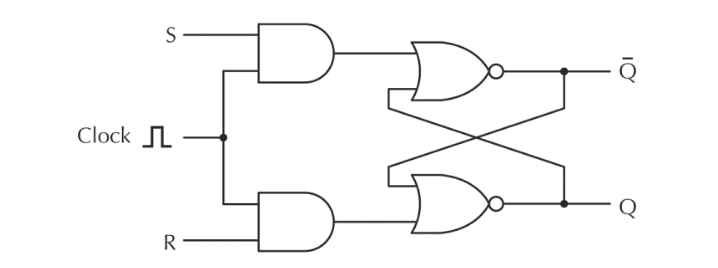
\includegraphics[width=0.75\linewidth]{LatchSRtemporizzato.png}
    \caption{Latch SR temporizzato}
    \label{Ltemp}
\end{figure}

\begin{figure}[H]
    \centering
    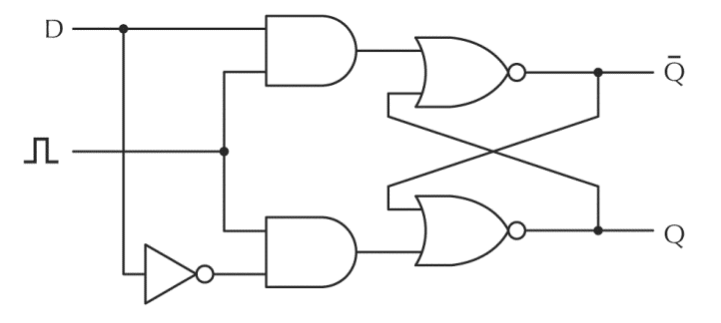
\includegraphics[width=0.75\linewidth]{latchDtemporizzato.png}
    \caption{Latch D temporizzato}
    \label{ldtemp}
\end{figure}

\begin{figure}[H]
    \centering
    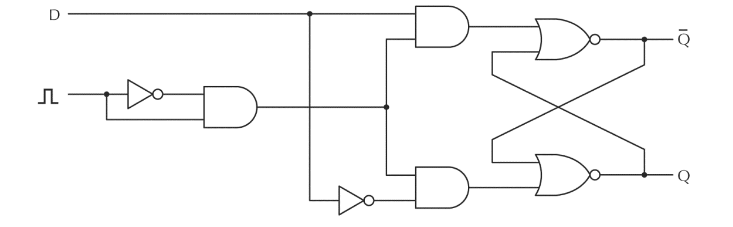
\includegraphics[width=0.75\linewidth]{Flip flop D.png}
    \caption{Flip-flop D}
    \label{ffd}
\end{figure}


\begin{figure}[H]
    \centering
    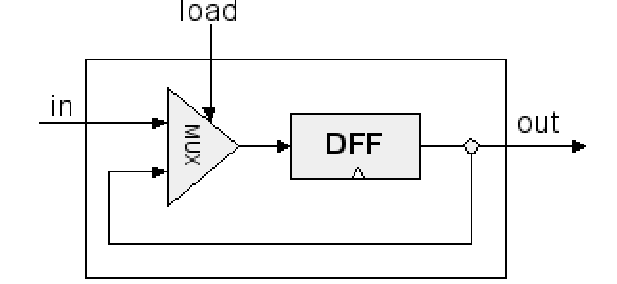
\includegraphics[width=0.75\linewidth]{1bitmeme.png}
    \caption{Schema di una memoria di 1 bit}
    \label{1bmem}
\end{figure}

\paragraph{Counter} Funziona come un registro di memoria ma ha un ulteriore modalità di incremento ed è utilizzato per realizzare il \textbf{Program counter}. Se reset = 1 è tutto zero, se reset = 0 si guarda il load e se load = 1 in output si manda l'input mentre se è 0 si guarda l'inc che se è 1 si incrementa di uno rispetto all'input. Se invece è tutto zero semplicemente si da in output il dato precedente in memoria.

\paragraph{Memoria con n-locazione} Avendo n-locazioni é presente un address bus che stabilisce quale indirizzo di memoria bisogna leggere e un load che quando é attivo sovrascrive la cella di memoria. Cosa importante é che il bus di indirizzo ha $log_2(n)$ bits perché deve solo codificare per il numero totale di indirizzi.

\paragraph{RAM} Essa è composta da n registri e attraverso un tot di multiplexer si scrive la cella di memoria indicata dall'address bus. Oltre a ciò bisogna sempre gestire il flusso output della RAM e per questo ed altri motivi può essere utile implementare circuiti combinatori prima e dopo circuiti sequenziali.

\begin{figure}[H]
    \centering
    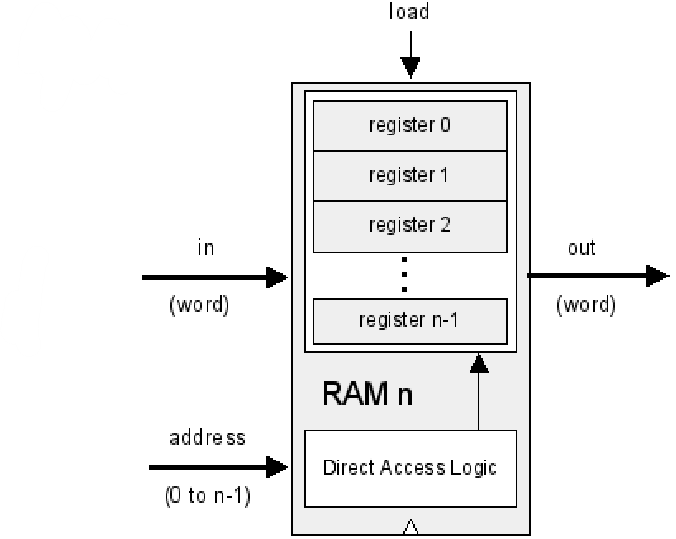
\includegraphics[width=0.60\linewidth]{Ramn.png}
    \caption{Implementazione di una ram per HACK}
    \label{ramn}
\end{figure}

\section{Rappresentazione delle informazioni}

Ogni informazione gestita da un calcolatore viene codificata in binario ma più in generale, data una codifica in base $b$ è possibile rappresentare i numeri interi tramite cifre che vanno da $0$ a $b-1$ nella forma $\sum_{i = 0}^k d_i * b^i$.
In informatica le codifiche posizionali principali sono: \textbf{binaria} (base 2), \textbf{ottale} (base 8) e \textbf{esadecimale} (base 16) che usa le lettere come cifre superiori al $9$. Con la definizione si può tranquillamente convertire in decimale qualsiasi numero di qualsiasi base possibile.
[slide prof dal binario agli altri]
Per passare da base 10 a base 2 o qualsiasi altra base si usa il \textbf{metodo delle divisioni successive} ovvero fare la divisione intera tra il numero decimale e la base, registrare il resto e una volta arrivati a 0 come risultato della divisione si leggono i resti dall'ultimo al primo e si ottiene il numero nella base desiderata. Un altro modo per passare da una qualche base b alla base 10 si parte da un somma = 0 che si moltiplica per la base e la si somma con la cifra nella posizione partendo da sinistra, reiterando si ottiene il risultato. 

Esempio di conversione:
$103_{(10)}$ = $1100111_2$ = $147_8$ = $67_{16}$


Per codificare i numeri interi nei calcolatori  ci sono diversi metodi:
\begin{itemize}
    \item \textbf{Modulo e segno}: il bit più a sx è usato per il segno (non c'è univocità perché esiste sia -0 che +0 e coi conti non va per nulla d'accordo es. -1 + 1)
    \item \textbf{Complemento a 1}: il bit più valente codifica comunque il segno, ma se il numero è negativo si scrive il suo complementare (es. 00000110 = 6 e 11111001 = -6) ma anche questo ha problemi con l'aritmetica
    \item \textbf{Complemento a 2}: si fa il complemento a 1 e si somma 1 tenendo in considerazione  tutti i riporti del caso questo porta l'aritmetica a funzionare meglio.
\end{itemize}

\paragraph{Numeri rappresentabili}
Con $k$ bit si possono rappresentare $2^k$ numeri diversi, più precisamente $[0; 2^k -1]$ se non ho segni, con segno oppure complemento a 1 $[-2^{k-1}+ 1; 2^{k-1} - 1]$ mentre in complemento a 2 $[-2^{k-1}; 2^{k-1} - 1]$.


\paragraph{Focus complemento a 2}: dato un numero $n$ rappresentabile come $b_{k-1} … b_0$ in complemento a 2 con $k$ bit, ottengo un numero che convertito in decimale é: $2^k -n$. Piú in generale data la sequenza $b_{k-1} … b_0$ in complemento a 2, il suo corrispettivo è -$b_{k-1} * 2^{k-1} + \sum ^{i=k-2} _0   b_i * 2^i$.	

\begin{figure} [H]
    \centering
    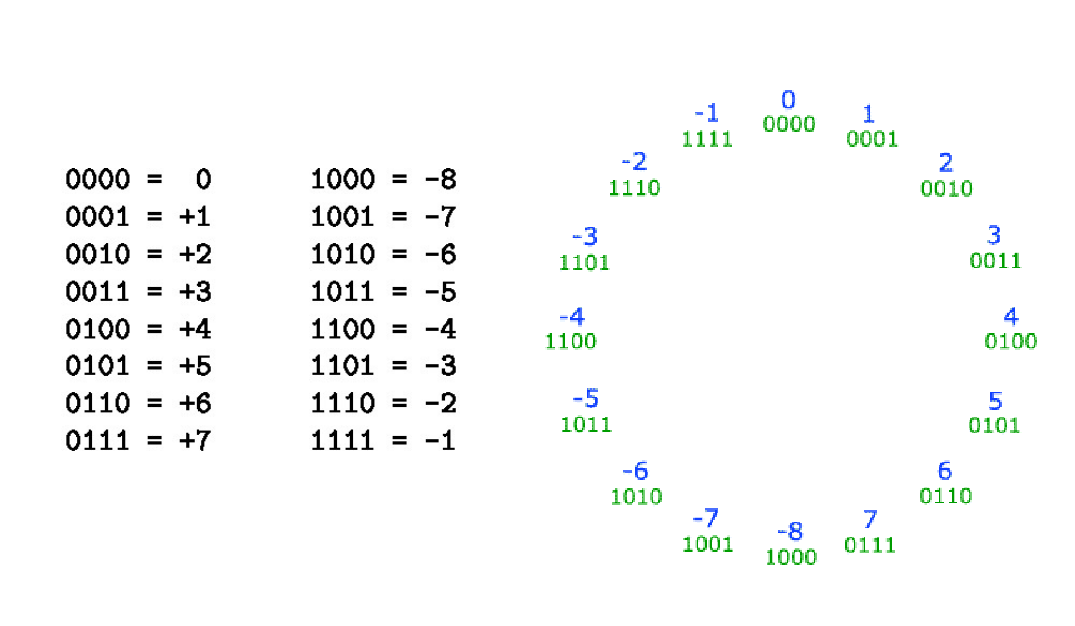
\includegraphics[width=0.85\linewidth]{ofc2.png}
    \caption{Esempio di come funziona l'overflow in complemento a 2}
    \label{ofc2}
\end{figure}

\paragraph{Codifica in eccesso} serve per rappresentare lo stesso intervallo del complemento a 1 ma shiftato tutto nei numeri positivi andando a sommare sempre $2^{k-1}$ a tutti i numeri.

\paragraph{Somma binaria tra due numeri} si esegue come le somme in colonna tra decimali prestando attenazione che 1 + 1 = 0, riporto di 1. Questo implica che le somme possono andare in overflow, mentre le sottrazioni in complemento a 2 non hanno alcun problema col riporto.

\begin{figure} [H]
    \centering
    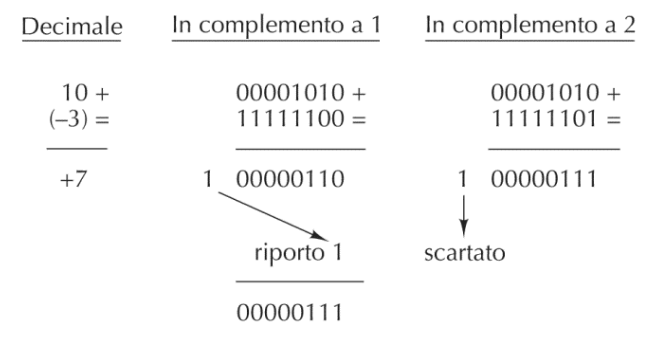
\includegraphics[width=0.75\linewidth]{somma bin.png}
    \caption{Esempio di somma in complemento a 1 e a 2}
    \label{somma bin}
\end{figure}

\paragraph{Rappresentazione in virgola mobile} é stata introdotta perché la rappresentazione dei numeri con la virgola fissa non è sempre efficace (es. $3*10^9$) quindi la virgola mobile li codifica in $n = f*10^e$ con $f$ \textbf{mantissa} (o frazione) e $e$ come esponente (o caratteristica).
La notazione floating point standard è stata decretata nello \textbf{standard IEEE 754} che definisce le precisioni nel single (binary 32) e double (binary64), nel primo caso:
\begin{itemize}
    \item 1 bit segno
    \item 8 bits esponente
    \item 23 bits mantissa con però codifiche particolari per NaN (not a number) e infiniti
\end{itemize}


\paragraph{Codice ASCII}
Molto versatile perché assegna valori alle lettere secondo l'ordine alfabetico il che rende molto facile shiftare da maiuscole e minuscolo e ordinare secondo l'ordine alfabetico. Inizialmente erano da 7 bit ma per necessità globali (i calcolatori sono stati aperti a culture con caratteri diversi rispetto a quelli anglosassoni) sono stati aumentati a 9 bit. In seguito è nata la codifica UNICODE che usa 16 bit, quindi è in continuità con il codice ascii, ma ne amplia i codici e inoltre ha dei codici "vuoti" che alla necessità possono essere riempiti, per esempio quando è nato l'euro il carattere non esisteva nella tabella così un codice vuoto gli è stato assegnato. Un problema è che usa due byte sia per un codice UNICODE, ASCII (7,8 bit) e a questo proposito è nato UTF-8 (Unicode Transformation Format) che ovvia al problema e usa da 1 a 4 bytes dipendentemente dal tipo di dato, i bit iniziali indicano che codice usare.

\paragraph{Codici correttori}
Avendo già un valore in binario con cui si vuole lavorare lo si deve trasportare e in alcuni casi questo porta ad errori, per questo motivo è necessario capire se il dato sia corretto o abbia un errore e per fare ciò si devono usare più bit di quelli necessari. Per esempio, volendo mandare 10 arriva 11,  per essere sicuro che all'arrivo si abbiano i due bit corretti mando 3 volte ogni bit per esempio 10 --> 111000.
Dunque, in base all'arrivo si capisce quali siano i bit mandati basandosi su quale sia la partenza più probabile; sempre nell'esempio di prima se arriva 101000 è più probabile che sia partito 111000 rispetto a 000000 perché nel secondo caso sarebbero stati commessi due errori rispetto ad uno solo nel primo caso. Nella realtà il processo è molto più efficiente: si usano meno bit e a questo proposito è importante introdurre la nozione di distanza di Hamming ovvero la distanza tra due sequenze di bit a livello di cambiamento degli stessi, per calcolarla si calcola il numero di bit diversi tra le due sequenze. Grazie a questa distanza se voglio rilevare una quantità $d$ errori ho bisogno di un codice con distanza di Hamming $>= d+1$ (per come funziona la gerarchia rispetto all'arrivo se voglio rilevare 2 errori ho bisogno di una sequenza di bit ricevuta che abbia la distanza di Hamming minima che sia maggiore di 2, se no potrebbe essere un altro codice equiprobabile e non si capirebbe se c'é l'errore o meno), se però si vuole correggere questo errore, e non soltanto sapere che c'è stato, sono necessari 2d + 1 bit.

\paragraph{Bit di parità}
E' uno dei codici più semplici e consiste nell' aggiungere un bit al messaggio originario e metterlo a 1 solo se avendo anche quello a 1 il numero di 1 è pari in tutto il codice; ha distanza di Hamming uguale a 2 dunque rivela 1 errore ma ne corregge 0.

\paragraph{Codice di Hamming} allosfrutta in modo intelligente diversi bit di parità. Esempio m = 16,  r = 5 (con 5 bit di controllo per correggere un errore)

\begin{center}
    \begin{tabular}{|c|c|c|c|c|c|c|c|c|c|c|c|c|c|c|}
        \hline
        0	& 0	& 0	& 0	& 0	& 0	& 0	& 1	& 1	& 1	& 1	& 1	& 1	& 1	& 1 \\
        0	& 0	&0	&1	&1	&1	&1	&0	&0	&0	&0	&1	&1	&1	&1 \\
        0	&1	&1	&0	&0	&1	&1	&0	&0	&1	&1	&0	&0	&1	&1 \\
        1	&0	&1	&0	&1	&0	&1	&0	&1	&0	&1	&0	&1	&0	&1 \\
        \hline
    \end{tabular}
\end{center}

Si prendono le colonne con un solo 1 e nel messaggio mandato in quelle posizioni si usa un bit di parità rispetto a tutte le colonne in cui c'è 1 in quella riga; rispetto al messaggio di partenza le colonne con i bit di parità sono saltate.

Quanto bisogna pagare per correggere gli errori? ovvero, inventando un codice come posso capire quanto è efficiente?

Con $m$ bit di dati e $r$ di controllo, quanto deve essere grande $r$ per correggere 1 errore?
In totale ho $m+r$ bit (che chiamo $n$),  dunque posso avere totalmente $2^m$ parole di partenza e ognuna ha 1 modo giusto e n modi sbagliati che devono essere diversi tra di loro ($n$ sono dunque le combinazioni possibili di bit cambiati rispetto alla parola iniziale). 
Ne viene che per correggere un errore $(n+1)*2^m <= 2^n$ da cui deriva che $2^r >= m + r + 1$. A questo punto bisogna trovare l'intersezione tra le due funzioni che in modo analitico non é affatto facile ma in questo caso si può andare per tentativi perché il numero di bit é naturale

\paragraph{Codice di Hamming generalizzato} lascio vuote le posizioni potenze di 2, poi riscrivo in binario le varie posizioni e i bit vuoti sono di parità rispetto agli "1" con quel bit "acceso nel numero" (similmente all'esempio precedente). Usando la formula di prima si capisce che il codice di Himming è il metodo più efficiente.

Come si decodifica? si ricontrollano i bit di parità se sono giusti allora la parola è per forza giusta se invece piú di un bit di parità é sbagliato significa che il bit con posizione che é la somma delle posizioni dei bit di parità errati sarà il bit errato. Nel caso di un solo bit di parità errato é lui quello sbagliato dell'intero messaggio.


\section{La ALU dell'architettura HACK}

\begin{figure}[H]
    \centering
    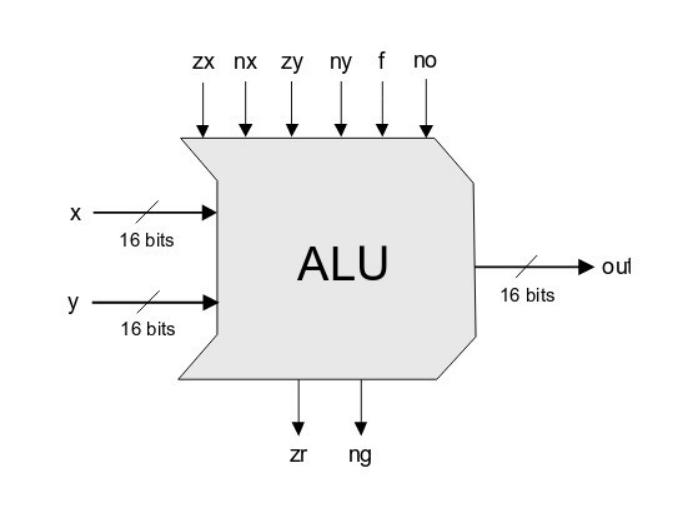
\includegraphics[width=0.9\linewidth]{esempioalu.png}
    \caption{Esempio schematico dell'ALU}
    \label{alues}
\end{figure}


Permette di fare, con uno sforzo maggiore di programmazione, tutto quello che può fare un'ALU normale nonostante sia meno elaborata a livello hardware, per HACK si intende un'architettura che lavora a 16 bit.
I sei input in alto sono i bit che indicano le operazioni da fare, mentre gli output in basso sono i \textbf{bit di stato} cioé zero e negativo per la traccia di quello che è successo durante l'esecuzione del programma.
Inoltre ha \textbf{2 registri a 16 bit}, il registro A è detto memory registr address perché memorizza l'indirizzo da cui andare a prendere le informazioni e l'\textbf{Adder} ovvero un circuito che serve a sommare due interi a complemento a 2. Usualmente si scompone il problema con un \textbf{Half adder} che somma 2 bit con riporto per poi successivamente avere il \textbf{Full adder} che somma 3 bit.
Per selezionare l'operazione da fare il processore HACK prende le parti simili per ogni operazione che si deve realizzare secondo la tabella (Fig.\ref{tabalu}): n e z lavorano singolarmente su gli input, mentre f regola l'operazione (solo adder e and logico) poi la no lavora sull'output. Quindi le 18 operazioni necessarie al funzionamento del processore HACK si risolvono in 3 circuiti diversi, che sono molto complessi ma ne giova la grandezza totale del circuito

 \begin{figure}[H]
     \centering
     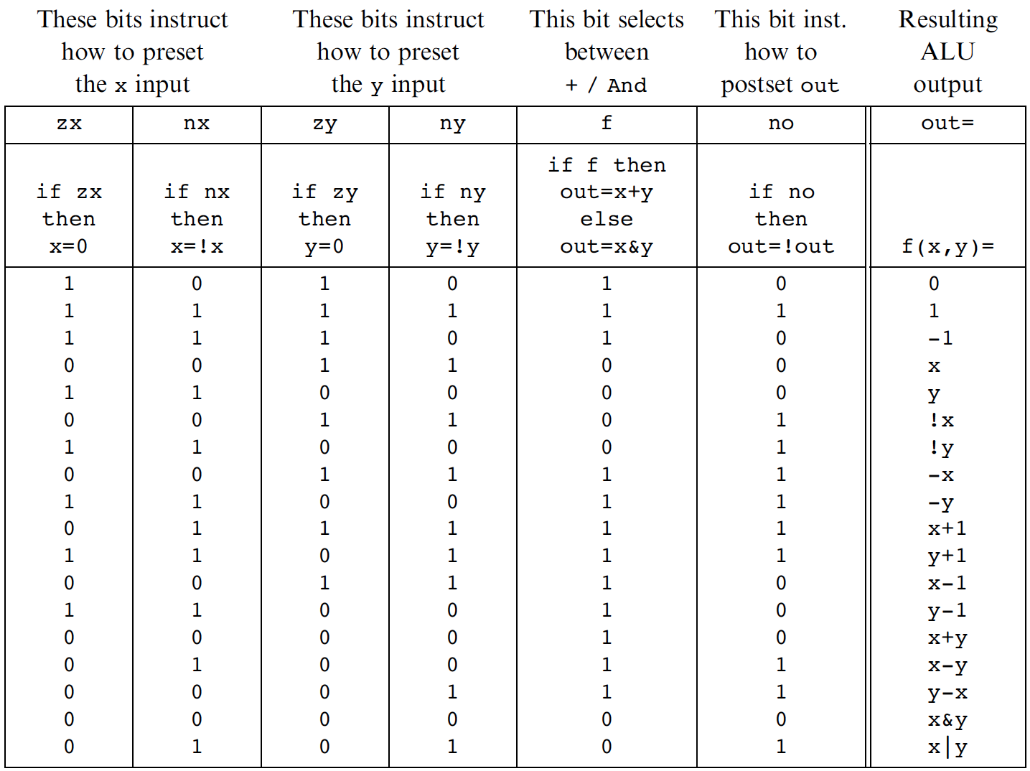
\includegraphics[width=1.15\linewidth]{tablealu.png}
     \caption{Operazioni aritmetico-logiche dell'ALU rispetto agli input}
     \label{tabalu}
 \end{figure}


\begin{figure}[H]
    \centering
    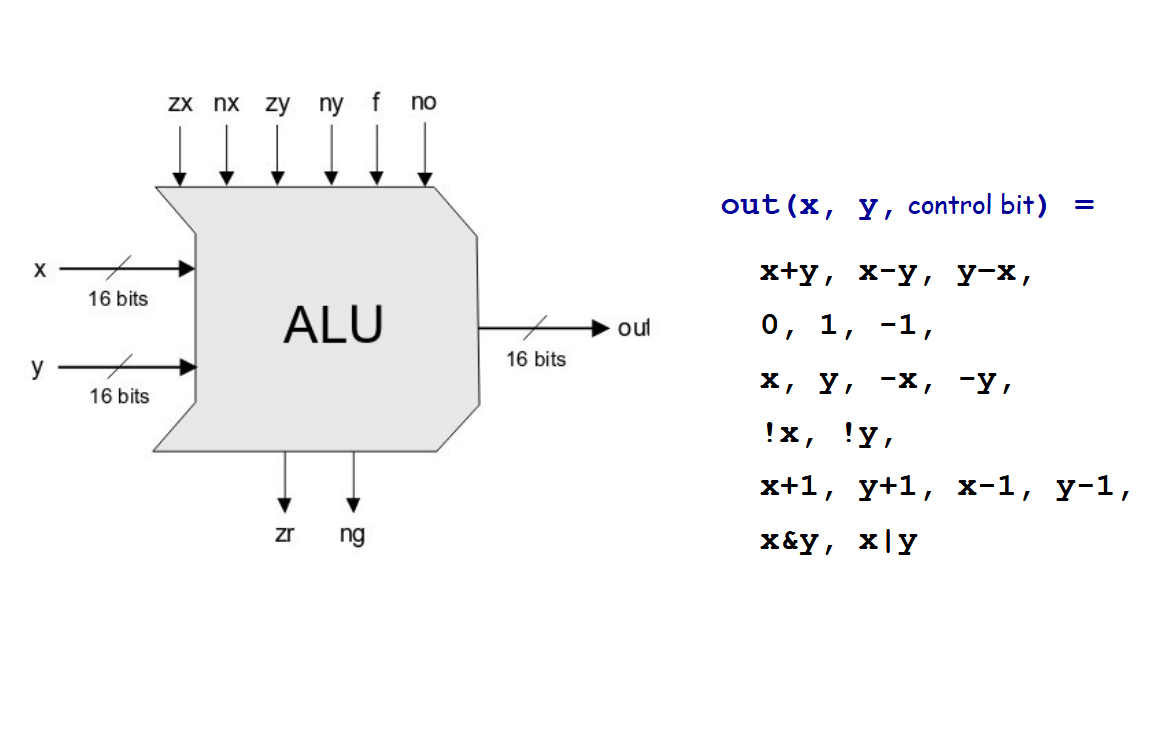
\includegraphics[width=1.15\linewidth]{ALUIO.png}
    \caption{Operazioni realizzabili con un ALU}
    \label{Aluletsgoski}
\end{figure}



%altra parte nuova (sempre da mettere a posto)

\section{Microarchitettura}
Descrive come comporre tra di loro i vari componenti per poter creare un calcolatore funazionante; schematicamente il funzionamento può essere riassunto in: lettrua dati dalla memoria, esecuzioni dei calcoli secondo le istruzioni del codice e produzione quindi di un output.

\textbf{N.B} l'architettura HACK è a 16 bit e usa la codifica a complemento a 2.

\begin{figure} [H]
    \centering
    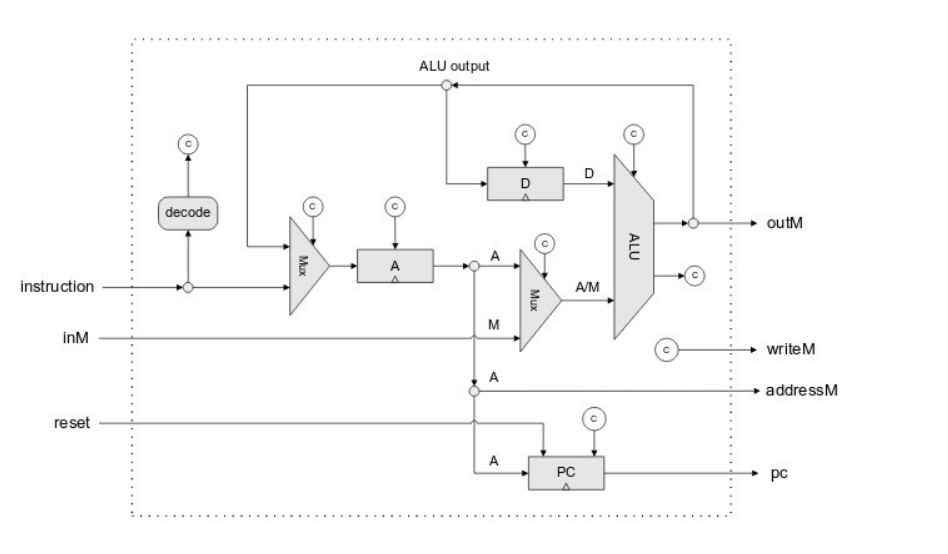
\includegraphics[width=1\linewidth]{microarchitettura HACK.png}
    \caption{Microarchitettura HACK}
    \label{fig:placeholder}
\end{figure}

I dati su cui lavora il processore vengono o dal \textbf{registro D}, da un multiplexer che gestisce il \textbf{registro A} oppure dall'\textbf{input M} che a livello assembly è gestito come registro interno. Il \textbf{program counter} scrive dei dati in memoria ma prende i dati anche da A che ha almeno 3 utilizzi (dato, indirizzo di memoria e momoria per il program counter). Il decode dell'istruzione gestisce praticamente tutti i componenti del processore perchè è come "selettore" in tutti i chip. L'architettura HACK è anche pensata per fare un'istruzione in un singolo ciclo di clock; le memorie fatte usando DFF e sono chiamate SRAM: sono le più veloci ma anche le più dispendiose per singolo bit di memoria e per questo sono state inventati altri tipi di memoria tipo la DRAM (che memorizza per piccole frazioni di secondo) in modo da bilanciare meglio il tempo di accesso su costo per bit memorizzato.


\paragraph{La cache} Abbiamo già introdotto questo componente, in questa sezione ne si approfondirà il funzionamento a livello di microarchitettura. L'idea di cache in realtà è talmente vincente che viene usata più volte nei calcolatori moderni:
\begin{itemize}
    \item \textbf{L1}: si trova direttamente nel chip della CPU ed è separata in una parte per le istruzioni e una per i dati (è la meno capiente delle 3).
    \item \textbf{L2}: si trova fuori dal processore ma nella stessa scheda dello stesso (leggermente più capiente).
    \item \textbf{L3}: fuori anche dalla scheda della CPU è la più capiente ma anche la più lenta delle 3.
\end{itemize}

\paragraph{Località temporale e località spaziale} Per \textbf{località temporale} si intende l'alta probabilità che si acceda più volte a breve distanza di tempo alla stessa locazione di memoria, per cui convinee tenere in cache il contenuto della memoria acceduta di recente. Mentre per \textbf{località spaziale} si intende l'alta probabilità che celle di memoria vicine a quella acceduta vengano accedute a breve distanza di tempo, dunque è utile trasferire in cache locazioni di memoria contigue a quella appena acceduta in modo tale da accedervi più facilmente (esempio degli array che sono locazioni contigue).

\paragraph{Direct Mapped Cache} Da immaginarsi come una tabella con 2048 righe a 32 byte e ha 3 colonne:

\begin{figure} [H]
    \centering
    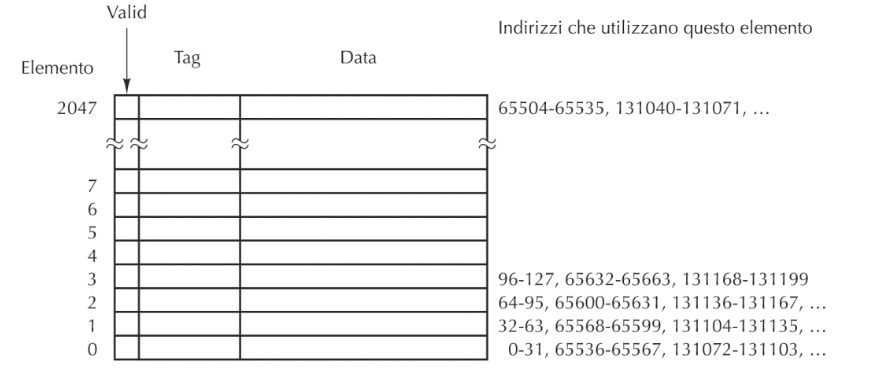
\includegraphics[width=1.1\linewidth]{Direct mapped cache esempio.png}
    \caption{Visualizzazione della Direct Mapped Cache}
    \label{Direct mapped cache}
\end{figure}


\begin{itemize}
    \item \textbf{Valid}: indica se la chace contiene o meno un blocco dati in quella riga.
    \item \textbf{Tag}: indica l'indirizzo ram del dato della riga in questione.
    \item \textbf{Data}: è effettivamente il dato.
\end{itemize}

Può essere molto utile guardare l'esercizio che abbiamo fatto riguardo alla cache su virtuale.


E' interssante il problema che si crea avendo un elaboratore multi-processor con una cache per ogni CPU ma un'unica memoria: quando una CPU modifica i dati nella propria cache lo stesso non avviene nella memoria condivisa dunque se le alre CPU dovessero fare operazioni su il dato modificato solo in una cache locale il risultato sarebbe sbagliaro. Per ovviare il problema o si crea una cache condivisa tra tutte le CPU (come viene fatto nella realtá) oppure serve un controllore, che sarebbe principalmente software, per gestire eventuali conflitti del genere.


\paragraph{Paginazione} Altra possibile soluzione al problema della gerarchia di memoria che gestisce il rapporto RAM $\leftrightarrow$ SSD similmente al rapporto cache $\leftrightarrow$ RAM. L'algoritmo di paginazione può essere meno efficiente e risultare comunque più veloce di un accesso in memoria ma un pagefoult implica molto tempo per reperire il dato; per questi motivi si usano algoritmi più raffinati di quelli della cache.

\paragraph{Pre-fetch istruzioni} Nonostante la cache sia veloce può comunque rappresentare, insieme alla RAM, un bottle-neck di velocità di computazione per questo l'idea è quella di, tenendo presente che le istruzioni molto spesso sono successive tra loro, caricare nella CPU l'istruzione successiva a quella che si sta eseguendo così che una volta finita si abbia un bel risparmio di tempo. Non sempre però questo si avvera e nel caso l'istruzione dopo non sia quella successiva si perde comunque tempo ma nel momento i cui si ha già pronta l'istruzione da eseguire si raddoppia la velocità.

\paragraph{Pipeline} Già solo il pre-fetch con un'unità a parte è un principio di pipeling, una struttura abbastanza semplice di pipeline può essere:

FETCH $\rightarrow$ DECODE $\rightarrow$ OPERANDI $\rightarrow$ ESECUZIONE $\rightarrow$ RISULTATO
Questa soluzione velocizza molto la computazione tranne nel caso in cui le istruzioni saltino tra di loro (\textbf{salti incondizionati}), si può leggermenta ovviare al problema rendendosi conto del salto il prima possibile creando una \textbf{bolla del pieline}. Oltre i salti incondizionati un'altra problematica per il pipeling sono i \textbf{salti condizionati} ovvero le situazioni in cui i salti dipendono da una condizione, un esempio di questo evento è un if-else nel programma oppure un ciclo. Per ovviare la problematica si può "tirare ad indovinare" e per capire ciò mentre si decodifica l'istruzione si usano euristiche tipo saltare all'indietro è più probabile di saltare in avanti (sempre nell'esempio di essere in un ciclo, tornare all'inizio è molto più probabile di andare avanti).

Un altro problema di questo sistema è il \textbf{Read After Write} ovvero il dover usare a tempo ravvicinato gli stessi registri (anche solo 1 in realtà), questo implica che potrebbero esserci dei casi in cui si leggono risultati vecchi perchè quelli aggiornati non sono ancora stati caricati in memoria ma il valore della locazione è richiesto. Anche in questo caso per evitare ulteriori problematiche i computer più semplici si rendono conto della problematica e aspettano creando una bolla del pipeling; i computer più moderni sono più "svegli" e mandano avanti operazioni successive facendo però attenzione che questa operazione non comprometta il codice. In generale però sono i programmatori o addirittura i compilatori ad accorgersi che il software può essere ottimizzato (\textbf{unrolling}).

\section{Instruction Set Architecture (del processore Hack)}
Si mettono insieme i componenti già studiati e assemblati perchè essa è l'interfaccia tra hardware e software dunque si basa su come sono stai collegati e costruiti i componenti. Per esempio, per utilizzare un processore lo si deve programmare con uno specifico \textbf{linguaggio assembly} costituito da un "\textbf{instruction set}" ovvero le istruzioni possibili del linguaggio; esso ovviamente è un linguaggio di \textbf{basso livello} in cui ogni istruzione del programma corrisponde ad un'operazione eseguibile dalla macchina a livello del circuito. Ci sono due tipi di assembly: quello simbolico leggibile dall'umano e il binario comprensibile dal computer, per tradurre l'uno nell'altro serve l'\textbf{assemblatore}. Per approcciarsi alla realizzazione di un elaboratore ci sono due tipi di approccio:
\begin{itemize}
    \item \textbf{RISC} (Reduced Instruction Set Computer): che utilizzano instruction set in cui ogni singola istruzione è più semplice, con lo scopo di consentire una implementazione hardware ottimizzata (nonostante i programmi diventino in generale più lunghi).
    \item \textbf{CISC} (Complex Instruction Set Computer): per sfruttare un instruction set più elaborato (che quindi permette di scrivere singole istruzioni che possono richiedere anche computazioni complesse).
\end{itemize}

Il processore HACK non è categorizzabile in questi due tipi perchè ha scelte miste volte alla didattica e soprattutto in questo processore ci sono 2 caratteristiche importanti: tutte le istruzioni sono implementate a livello hardware ed avvegono tutte in un singolo ciclo di clock.

\subsection{Il computer HACK}
\begin{itemize}
    \item Data Memory: registri a 16 bit per salvare i dati di lavoro, include principalmente la RAM
    \item Instruction Memory: composta da registri anch'essi a 16 bit con le istruzioni del programma, è in sostanza la ROM.
    \item Registri: \begin{itemize}
        \item \textbf{D} e \textbf{A}: i due registri interni della CPU, il primo direttamente collegato alla RAM e il secondo alla ROM
        \item \textbf{M}: Data memory attualmente puntato dal registro A (MEM[A]).
    \end{itemize}
    \item \textbf{ALU}: esegue le computazioni
    \item \textbf{Program Counter}: registro che contiene l'indirizzo della ROM con la prossima istruzione da eseguire
\end{itemize} 

\subsection{Tipi di istruzioni}
\begin{itemize}
    \item \textbf{A-instruction}: si limitano a caricare un valore all'interno del registro A.
    \item \textbf{C-instruction}: sono istruzioni che coinvolgono la computazione e usano \textbf{sempre} la ALU (a differenza delle A-instruction). Le computazioni eseguibili sono: 
    \begin{figure}[H]
        \centering
        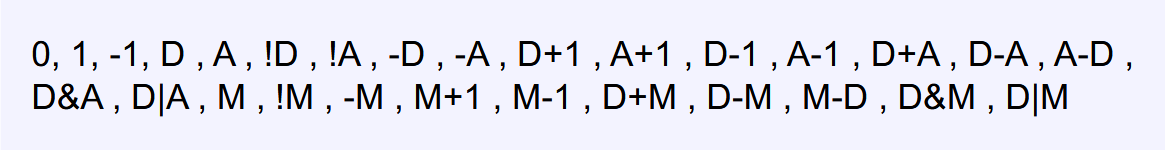
\includegraphics[width=1\linewidth]{Hack instruction.png}
        \caption{Possibili computazioni}
        \label{comphack}
    \end{figure}
\end{itemize}

\subsection{C-instruction}
\begin{center}
    Forma generale: \textit{dest = comp ; jump}
\end{center}
\begin{itemize}
    \item \textbf{comp}: è la computazione da eseguire
    \item \textbf{dest}: è la cella di memoria dove memorizzare il risultato
    \item \textbf{jump}: specifica se dopo aver eseguito \textit{dest = comp} bisogni saltare nell'esecuzione del programma ovvero aggiornare il contenuto del PC al valore che è \textbf{attualmente salvato nell'indirizzo A}. Molto importante il salto viene fatto dopo ad aver confrontato il risultato della computazione con 0 (zero). Nel caso della nostra architettura basa guardare i due output \textbf{zr} e \textbf{ng}. Le derettive a questo punto sono: \begin{itemize}
        \item \textbf{JGT}: jump if grater than
        \item \textbf{JEQ}: jump if equal
        \item \textbf{JGE}: jump if grater or equal
        \item \textbf{JLT}: jump if less than
        \item \textbf{JNE}: jump if not equal
        \item \textbf{JLE}: jump if less or equal
        \item \textbf{JMP}: jump always
    \end{itemize} 
\end{itemize}

\subsection{A-instruction}
\begin{center}
    Forma generale: \textit{@value}
\end{center}

con value che è un valore, la A-instruction però non usa la ALU e lavora ovviamente sul registro A.

\paragraph{Comparazioni non con 0}
Tutti i test sono fatti confrontando con 0, quindi per fare un confronto con un numero diverso si risolve la dis/equazione.


\subsection{Etichette} 
Non sono strettamente necessarie ma permettono di mettere dei "segnalibri" ai punti del programma, sono dichiarate tra parentesi e non sono messe in locazione di memoria infatti l'assemblatore elimina le etichette e nei punti \textit{@ETICHETTA} viene sostituito l'indirizzo giusto (ovvero quello successivamente dopo l'etichetta). (Fig. \ref{eseti})

\begin{figure}[H]
    \centering
    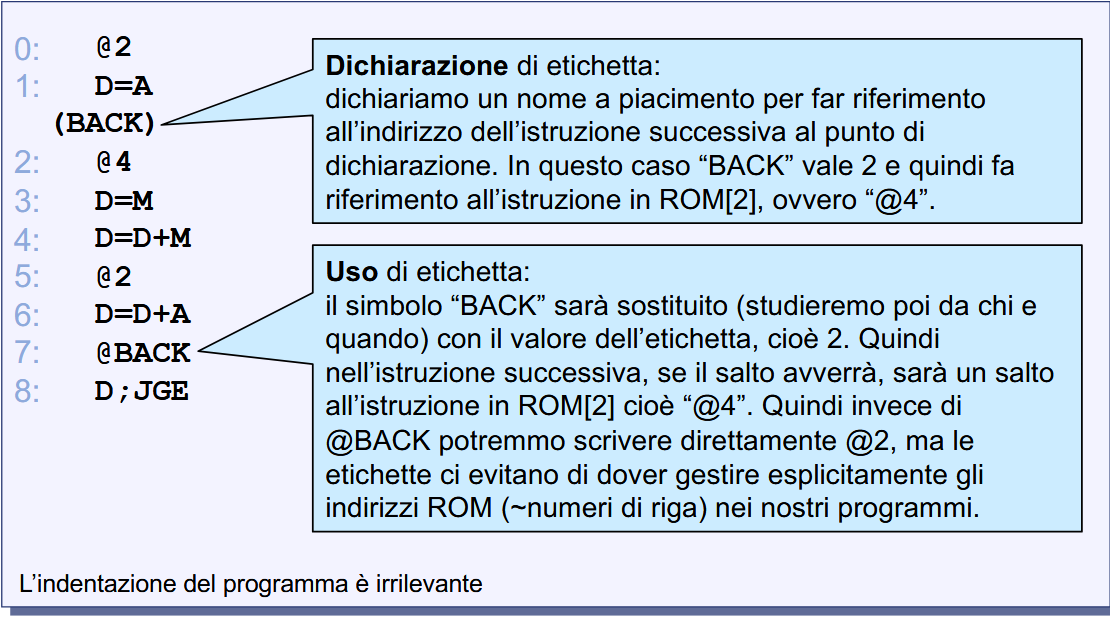
\includegraphics[width=0.95\linewidth]{esetichette.png}
    \caption{Esempio di utilizzo di etichette}
    \label{eseti}
\end{figure}

\subsection{Implementazione if then else}
\begin{figure}[H]
    \centering
    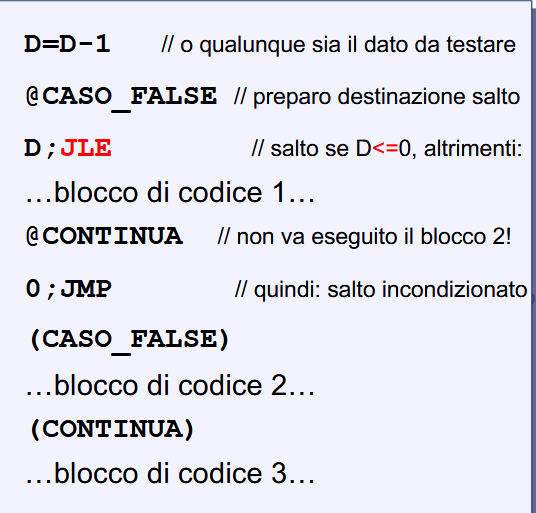
\includegraphics[width=0.5\linewidth]{ifthenelse.png}
    \caption{Implementazione costrutto if-then-else}
    \label{iifthenelse}
\end{figure}
Queste implementazione sfrutta le etichette ma soprattutto l'inversione della condizione: il blocco di istruzioni dentro all'if va eseguito solo nei casi in cui la condizione é vera, dunque il salto va eseguito solo nel caso in cui la condizione sia falsa (motivo per cui la condizione é invertita) nel punto in cui inizia il blocco di istruzioni dell'else.

\subsection{Implementazione while}
\begin{figure}[H]
    \centering
    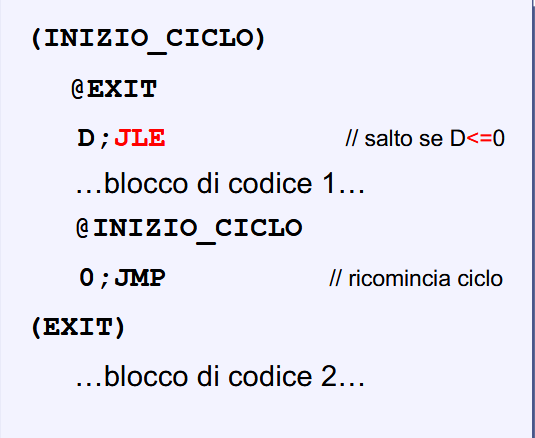
\includegraphics[width=0.5\linewidth]{while.png}
    \caption{Esempio implementazione del while}
    \label{while}
\end{figure}
L'implementazione del while é molto simile a quella dell'if se non che alla fine del blocco di istruzioni bisogna far saltare il programma all'inizio del corpo per ritestare la condizione.


\subsection{Variabili}
Sono utilizzate per fare riferimento ad indirizzo di memoria RAM ma non si ha controllo di dove vengano memorizzate. Ci sono due tipi di variabili:
\begin{itemize}
    \item \textbf{Pre-definite}: come SCREEN e KBD che sono pre impostate (la prima è la prima locazione di memoria che codifica per lo schermo, la seconda l'ultima che prende in input i tasti dalla tastiera).
    \item \textbf{Definite dall'utente}: sono variabili da 3 caratteri a cui l'assemblatore assegna il valore di una locazione di memoria in modo tale da poterci accedere tramite @var che però non rientrano tra MEM[0...15].
\end{itemize}


\subsection{Fine dei programmi}
Alla fine si fa un ciclo chiuso, perchè non esiste un costrutto di fine, che previene l'esecuzione di comandi successivi alla fine (non nel caso HACK).

\subsection{ISA non HACK ma di architetture più complesse}
A differenza dell'architettura HACK che prevede due tipi di istruzioni, in un generico computer le istruzione ISA contengono:
\begin{itemize}
    \item \textbf{Opcode} ovvero la parte che indica l'istruzione da eseguire
    \item \textbf{Operandi} su cui eseguire l'istruzione, ci si riferisce ad essi tramite indirizzi.
\end{itemize}
Per questo motivo, in alcuni casi, può succedere che la codifica non sia rigida come quella di HACK e che le varie parti descritte prima occupino più o meno bit di codifica, altre architetture possono contentere, in una singola \textit{word}, più istruzioni.
Altro aspetto centrale è la parte di indirizzamento perchè è ciò che indica gli operandi su cui operare, esistono diversi metodi di indirizzamento:
\begin{itemize}
    \item \textbf{Immediato}: l'istruzione contiene già l'oprando da usare
    \item \textbf{Diretto}: l'istruzione contiene l'indirizzo di memoria completo dell'operando da utilizzare.
    \item \textbf{A Registro}: l'operando è prelevato da un registro
    \item \textbf{A registro indiretto}: L'indirizzo da cui reperire l'operando è contenuto in un registro.
    \item \textbf{Indicizzato}: si include un \textit{offset} da sommare ad un registro ottenendo così l'indirizzo dell'operando.
    \item \textbf{Stack}: simile a quello indicizzato perchè usa un \textit{pila LIFO} e quindi per guardare i vari elementi si usa comunque un offset per andare a vedere il dato elemento della lista.
\end{itemize}

Esisitono inoltre istruzioni come \textbf{CALL} che chiamano delle procedure, esse interrompono l'esecuzione del codice in modo sequenziale per andare in un altro indirizzo di istruzione. Alla fine della call ci sarà un \textbf{RET} all'esecuzione sequenziale, proprio come le funzioni di C++.  Per questo motivo è necessario isanziare in memoria un \textbf{record di attivazione} ovvero uno spazio di memeoria con tutti i dati necessari all'esecuzione della procedura, questi record di attivazione sono organizzati a pila secondo la politica \textit{LIFO}. Una volta terminanta la funzione 2 sono le informazioni che ci servono sapere: l'inizio del record corrente (\textbf{FP}) e l'inidrizzo che punta alla testa dello stack (\textbf{SP}). Per \textbf{stack} si intende lo spazio di memoria in cui sono impilati i vari record di attivazione. Inoltre ogni record di attivazione ha una uno spazio di memoria che é riservato a memorizzare il \textbf{vecchio FP} in modo che, una volta terminata l'esecuzione, si deve aggionare l'\textbf{FP} e decrementare lo \textbf{SP}. Oltre a queste informazioni, generalmente alla chiamata di una procedura vengono salvati:
\begin{itemize}
    \item Parametri di invocazione
    \item Indirizzo di ritorno
    \item Vecchio FP
    \item Variabili locali
\end{itemize}

\subsubsection{Trap}
E' una chiamata di una procedura automatica quando si verificano certi tipi di errori come Opcode non definito (istruzione sconosciuta), accesso ad un area di memoria non consentita al programma o overflow. A questo punto un'unità di controllo specifica riceve il segnale e il \textbf{gestore di trap} grazie alla CPU e all'OS stabilisce se fare dei salti nel programma oppure continuare normalmente l'esecuzione. Molto importante è il fatto che il \textbf{trap} è \textbf{sincrono} al programma, ovvero è un'istruzione del programma che genera il segnale di trap e che quindi alleggerisce il lavoro del programmatore che delega al sistema la gestione dei casi trap.

\subsubsection{Interrupt}
Similmente alle trap queste istruzioni interrompono il programma in esecuzione e trasferisce il controllo ad un gestore deputato (\textbf{ISR}: Interrupt Service Routine), questo tipo di segnali sono solitamente legati ai dispositivi di input/output e possono riguardare eventi e non solo possibili errori.


Esempio: in generale, nel caso di dispositivi, si usano dedicate linee per la notifica di un interrupt (interrupt requests), che vengono ricevute da un circuito di controllo il quale invia un segnale alla CPU. Quando la CPU è pronta (restituisce un acknowledgement della richiesta), il circuito scrive sul bus dati l’indice (interrupt vector) dell’ISR specifica per l’interrupt/dispositivo. Questo indice viene usato per prelevare l’indirizzo dell’ISR (dove il programma relativo è memorizzato) da una apposita tabella statica salvata in memoria (Interrupt Description Vector, a sua volta puntato da un registro specializzato – vedi indirizzamento indicizzato), così che la CPU può salvare lo stato corrente e settare il program counter a quell’indirizzo (effettuando così una chiamata di procedura all’ISR specifico).
L'interrupt è fondamentale per evitare il \textbf{busy waiting} ovvero il controllare sempre se è accuduto un evento infatti è come se ne notificasse l'avvenimento, dunque gli interrupt sono \textbf{asincroni} rispetto al programma.

\subsubsection{Mascherabilità degli interrupt}
Ci sono certi programmi a cui non frega nienete dell'interrupt quindi in alcuni casi l'OS decide di \textbf{mascherare} gli interrupt per non fermare l'esecuzione del programma. In altri casi ancora possono essere dichiarati degli interrupt \textbf{non-mascherabili}.

\subsubsection{Priorità degli interrupt}
Si stabilisce una gerarchià degli interrupt dunque l'interrupt è efficace solo se è maggiore della priorità attualmente in gestione se no viene messo in attesa che quello più imposrtante sia finito.

\begin{figure}[H]
    \centering
    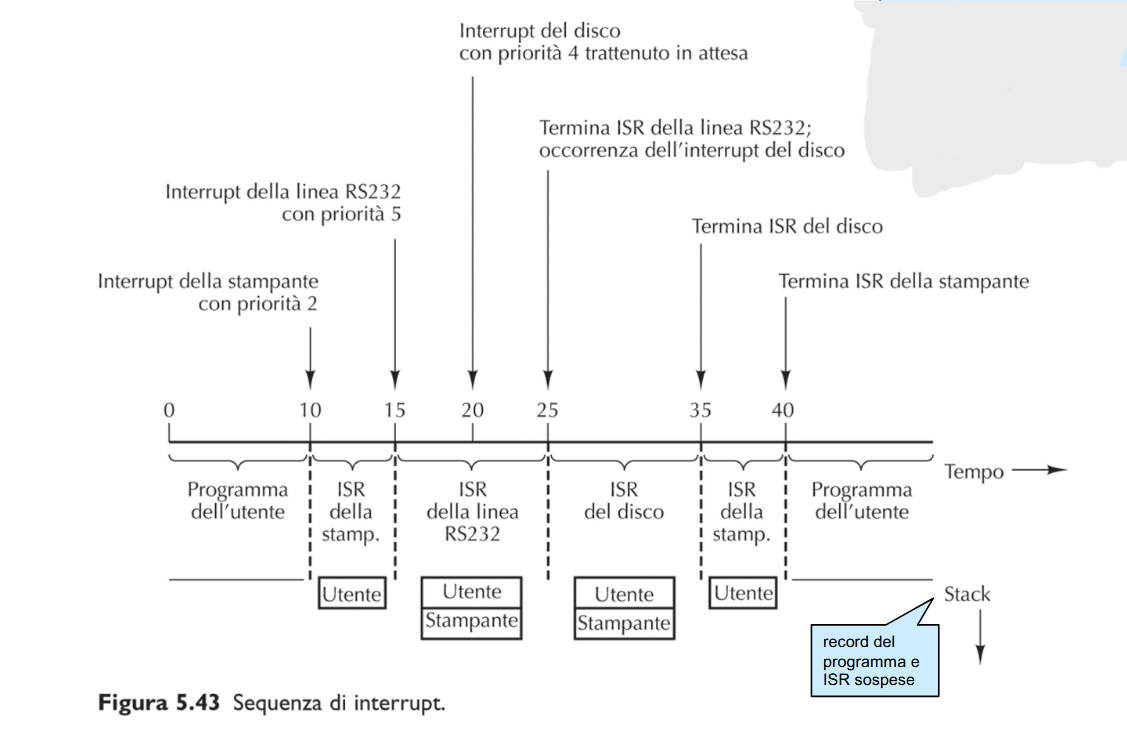
\includegraphics[width=0.85\linewidth]{interrupt priority.png}
    \caption{Esempio di gestione di interrupt di diverse prioritá}
    \label{intrprio}
\end{figure}




\section{Livello sistema operativo}
É un programma trasversale che gestisce l'hardware del calcolatore quindi la memoria, i processi (programmi in esecuzione), le periferiche... Le parti importanti dell'interfaccia del sistema operativo sono l'\textbf{IPC} (Inter Process Commands ovvero comandi che si passano tra i processi), lo \textbf{scheduling} per gli interrupt per esempio ma la parte piú importante é la \textbf{gestione della memoria}.

\subsection{Virtualizzazione della memoria}
E' uno stratagemma per far finta di avere molto più spazio di quello che si ha realmente a disposizione: consiste nel memorizzare parte dei dati nella memoria di massa e fare degli swapping continui tra memoria primaria e memoria secondaria in modo da avere in RAM solo i dati necessari alle operazioni che si stanno svolgendo nel dato momento. Questa complicazione non tange minimamente il singolo programma che si sta eseguendo, è gestita interamente dal sistema operativo per cui per il programma esso sta lavorando su celle di memoria cotigue. Un vantaggio a favore di questa strategia, oltre alla maggiore quantita' di spazio senza dover aumentare la capacitá fisica, é la compartimentazione della memoria tra i vari processi. Tra i contro c'è la maggiore lentezza della memoria secondarie e il lavoro in più: dato un \textbf{indirizzo virtuale} esso va \textbf{mappato} (tradotto) in un \textbf{indirizzo fisico} e gestire anche quali dati tenere nella RAM e quali nella memoria secondaria.
\subsection{Paginazione}
La memoria virtuale viene divisa in \textbf{pagine} equidimensionali, la RAM viene divisa in \textbf{blocchi} equidimensionali tra loro e le pagine; l'idea è quella di avere nei blocchi le pagine che si devono utilizzare in quel momento questo si fa attraverso le \textbf{tabelle delle pagine} gestite da un componente apposito chiamato \textbf{MMU} (Memory Menagement Unit). Nella tabella delle pagina c'è scritto se un certo indirizzo è salvato in RAM e se si dove. Nel caso ci sia un \textbf{Page fault} ovvero che l'indirizzo virtuale non ricade nella RAM ma nella memoria secondaria avverrà una page \textbf{swapping} ovvero si copia un blocco in una pagine e la pagine richiesta viene copiata in un blocco (la scelta avviene grazie ad un \textit{algoritmo di paginazione}). I due maggiori tipo di algoritmi di paginazione sono: \begin{itemize}
    \item \textbf{LRU (Least Recently Used)}: si rimuove il blocco che corrisponde alla pagina non acceduta da più tempo (tipo la lista). 
    \item \textbf{FIFO (First In, First Out)}: il blocco in memoria da più tempo è quello che viene sovrascritto
\end{itemize}

\subsubsection{Dirty bit}
Nel caso si debba liberare un blocco può essere furbo avere un modo di capire se la pagina è stata modificata in modo tale che se il blocco è stato solo letto non è necessario ricopiarlo nella rispettiva pagina. Per questo il \textbf{dirty bit} è un bit usato come booleano per vedere se è stata modificata.

\subsubsection{Implementazioni reali}
Le tabelle della pagine sono memorizzate in registri dedicati oppure è anch'essa salvata in memoria principale puntata però da un registro dedicato, in questo caso si ha anche un offset per sapere se la pagina è salvata in un blocco o meno.
Un'altra possibile implementazione è avere una cache associativa tra pagina virtuale e blocco di memoria fisica.

\subsection{Frammentazione interna} Supponiamo di avere un programma a cui serva una quantità di memoria che non è un multiplo della dimensione delle pagine quindi l'ultima pagina non viene mai completamente utilizzata. Questo fenomeno è detto \textbf{frammentazione interna}.

\subsection{Segmentazione}
E' un organizzazione \textit{logica} della memoria in porzioni (\textbf{segmenti}) che sono utilizzate in diverse modalità/scopi, diritto di accesso, ecc... e ogni segmento ha il proprio spazio di indirizzamento e logicamente è simile ad avere disponibili diverse memorie contemporaneamente. Ma a differenza della paginazione, la segmentazione non é trasparente rispetto al programma e questo porta, inoltre, anche ad avere la necessità di un doppio indirizzamento. Nella realtà questo problema è risolto attraverso dei \textbf{registri di segmento} che puntano alla base del segmento e dunque l'indirizzo fisico sarà la base del segmento + l'offset. Come nella paginazione si possono tenere solo alcuni segmenti in memoria ma swapping tra RAM e memoria secondaria puó creare delle \textbf{lacune} perchè i segmenti \textbf{non hanno dimesione fissa}. Il fenomeno di creazione di lacune viene indicata sotto il nome di \textbf{frammentazione esterna}. Per ovviare al problema si deve interropere l'esecuzione e colmare le lacune in modo intelligente secondo due famiglie di algoritmi, ovvero: \begin{itemize}
    \item \textbf{Best fit}: si inserisce il nuovo segmento nella lacuna più piccola che lo può contenere.
    \item \textbf{First fit}: si inserisce il nuovo segmento nella prima lacuna disponibile che lo può contenere.
\end{itemize} 
In realtà fino a pochi anni fa si faceva una \textit{paginazione della frammentazione} ovvero i vari segmenti erano divisi in pagine e si andava di paginazione, questo però comporta uno sforzo maggiore della \textbf{MMU} che deve avere una tabella dei segmenti e anche una tabella delle pagine per ogni segmento.

I moderni computer a 64 bit hanno una possibilità di indirizzamento talmente ampia che molti dei problemi che la segmentazione risolve non si presentano piú per cui non viene più usata, in questi casi si usa solo la paginazione.
Ci sono però 3 principali modalità di funzionamento di un architettura (in realtá queste modalitá possono interscambiarsi a seconda della necessitá, tipo l'avvio): \begin{itemize}
    \item  \textbf{Real mode}: i registri dei segmenti contengono l'indirizzo dell'inizio del segmento in memoria. No protezione degli accessi nè paginazione.
    \item \textbf{Protected mode}: c'è il \textbf{descrittore del segmento} che aggiunge informazioni, i puntatori del segmento puntano ad essi.
    \item \textbf{Long mode}: solo nei sistemi a 64 bit si elimina la segmentazione ma si mantengono solo 2 segmenti generici, la protezione della memoria è garantita dalla paginazione che è obbligatoria e multilivello (differenti tabelle di paginazione).
\end{itemize}

\subsection{Linking}
Quando si vuole eseguire un programma potrebbe succedere che si usino diversi file, questi diversi file vengono compliati in momenti diversi e vengono generati i file oggetto per ognuno di essi e quindi nasce il problema di mettere insieme tutti questi file, solitamente in modo contiguo, in modo da avere un eseguibile unico. Il \textbf{Linker} è il programma che collega tra loro questi file diversi e gestisce il problema che ogni file assembly si riferisce a indirizzi di linee locali alla singola procedura, per cui il linker serve principalmente a sistemare sia i \textbf{riferimenti interni}, ovvero i riferimenti a linee di codice all'interno della singola procedura, per cui effettua uno shift attreverso il \textbf{dizionario di rilocazione}, e i \textbf{riferimenti esterni} ovvero la chiamata ad altre procedure per cui è necessario una \textbf{tabella dei riferimenti esterni}. 
\subsection{Linking dinamico} In alcuni casi, alcune procedure, non vengono inserite nell'eseguibile ma vengono collegate \textbf{dinamicamente} al momento dell'esecuzione. Queste procedure sono per esempio programmi che si assume siano già scaricati nel computer, in modo da alleggerire l'eseguibile, e che spesso vengono aggiornati, in modo da non dover ri-linkare tutto il programma oppure sono driver di schede video. Per linkare dinamicamente si sfruttano i \textit{trap}: nel programma compilato si fa una chiamata ad un indirizzo volutamente sbagliato in modo tale che si generi il trap, quando si esegue il programma una volta arrivato alla chiamata sbagliata il gestore del trap andrà a cercare l'indirizzo della procedura e lo sostituirà a tutte le altre chiamate sbagliate all'interno del programma. 



\section{Virtual Machine per il computer HACK}
E' un modello astratto di calcolo e non fa riferimento ad una specifica architettura, costituisce un livello intermedio tra linguggio ad alto livello e il linguaggio assembly usato nel modello di compilazione a \textbf{2 livelli}:\begin{enumerate}
    \item Si compila il codice in un linguaggio intermedio che non dipende dall'architettura ma solo dal \textit{sorgente}.
    \item Dal linguaggio intermedio si passa a quello target che dipende dalla macchina.
\end{enumerate}
Impareremo dunque a programmmare in questo linguaggio intermedio che è molto simile all'assembly per HACK. Per manipolare i dati si usa una struttura a pila quindi se si vuole fare la somma tra due numeri bisogna prima impilarli, nel caso di operatori binari (2 operandi) considera per primo il penultimo nello stack e l'ultimo come secondo. Una volte terminata l'operazione gli operandi sono consumeti e viene lasciato sulla pila il risultato. Il pop di una pila rimuove l'ultimo elemento e lo può memorizzare in una certa porzione di memoria; la memoria della \textit{VM HACK} è segmentata e questo permette di distinguere logicamente la memoria, ci sono diversi segmenti: 
\begin{itemize}
    \item \textbf{Static}: variabili globali.
    \item \textbf{Argument}: argomenti con cui una funzione è stata chiamata.
    \item \textbf{Local}: argomenti locali alla funzione con cui può lavorare.
\end{itemize}

Nel codice se si volesse accere ad un segmento di memoria:
\begin{verbatim}
    pop segment addr //pop dalla cima dello stack, 
                     //salvando il valore in (segment, addr)
    push segment addr //push in cima dello stack del 
                      //valore all'indirizzo (segmento, addr)
\end{verbatim}

Esempio di esercizio $((5-1)+(4+2)) > (7+2)$
\begin{verbatim}
    push constant 5  // pila: 5
    push constant 1  // pila: 5, 1
    sub  // pila: 4
    push constant 4  // pila: 4, 4
    push costant 2  // pila: 4, 4, 2
    add  // pila: 4, 6
    add  // pila: 10
    push constant 7 // pila: 10, 7
    push constant 2 // pila: 10, 7, 2
    add // pila: 10, 9
    gt // pila: true
\end{verbatim}

Mentre se si vogliono implementare i gestori del flusso del programma:
 \begin{verbatim}
     // if local [0] > 3 then local[0] = 0
     push local 0
     push constant 3
     gt
     not
     if-goto ELSE
     push constant 0
     pop local 0
     goto END
     label ELSE
 \end{verbatim}


Per quanto riguarda l'implementazione delle funzioni per convenzione la funzione chiamante fa il push degli argomenti sulla pila poi fa la \textit{call} della funzione da chiamare e aspetta il ruturn. Prima di finire l'esecuzione, il \textit{chiamato}, deve fare la push del valore di ritorno, quindi l'effetto netto di una chiamata di funzione è la consumazione degli elementi (parametri) e la generazione del valore di ritorno. Molto importante è specificare sempre il numero di variabili locali.

Esercizio: implementarela seguente funzione in VM per HACK
\begin{figure} [H]
    \centering
    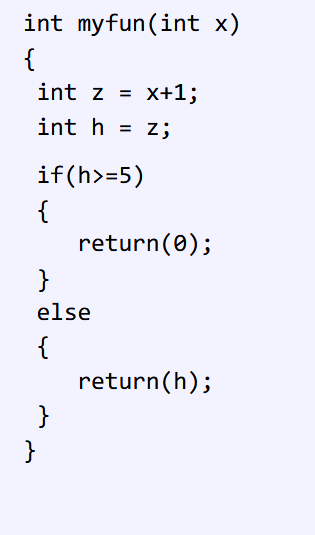
\includegraphics[width=0.35\linewidth]{esempio es VM.png}
    \caption{Funzione da implementare}
    \label{esVMen}
\end{figure}

\begin{verbatim}
    function dummy 1
    push constant 0
    pop local 0
    push argument 0
    push argument 1
    lt
    push argument 0
    push argument 1
    eq
    or
    if-goto ELSE
    push local 1
    return
    label ELSE
    push constant 3
    push local 1
    sum
    pop local 0
    push local 0
    push argument 0
    gt
    return
\end{verbatim}






Altro esercizio:

\begin{figure} [H]
    \centering
    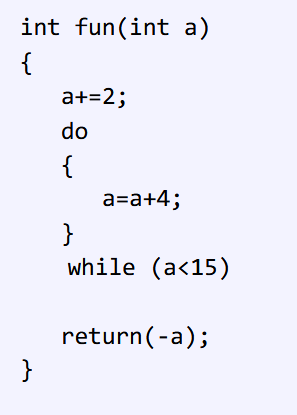
\includegraphics[width=0.35\linewidth]{altro es Vm.png}
    \caption{Esercizio 2}
    \label{nigger}
\end{figure}


\begin{verbatim}
    function fun 0
    push argument 0
    push constant 2
    add
    pop argument 0
    label INIZIO
    push argument 0
    push constant 4
    add
    pop argument 0
    push argument 0
    push constant 15
    lt
    if-goto INIZIO
    push argument 0
    neg
    return
\end{verbatim}



Altro esercizio
\begin{figure} [H]
    \centering 
    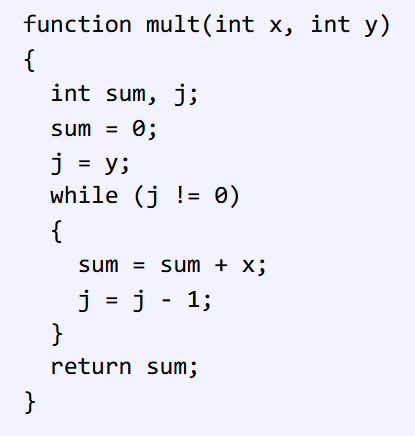
\includegraphics[width=0.40\linewidth]{ult es VM.png}
    \caption{Esercizio 3}
    \label{bigger digger}
\end{figure}

\begin{verbatim}
    function mult 2
    push const 0
    pop local 0
    push argument 1
    pop local 1
    label COND
    push local 1
    push constant 0
    eq
    if-goto END
    push local 0
    push argument 0
    add
    pop local 0
    push local 1
    push constant 1
    sub
    pop local 1
    goto COND
    label END
    push local 0
    return

    
\end{verbatim}



\end{document}


%\subsection{Esercizi}

5. 
@3
D = A
D = D+M

6.
@3
D = A
@4
D = D + A


7.
@7
D = A
@3
M = D

8. 
D = M
@3
D = D + A

1.2
@3
D = D - A

1.3
@10
D = A
@5
D = D - M

1.4
@2
D = A
@0
D = D + M


1.6
@0
A = M
D = M

1.7
@0
D = M
A = M
M = D


MEM[2] = MEM[0] + MEM [1]
@0
D = M
@1
D = D + M
@2
M = D

Esercizi sui salti:
1. se MEM[0]>0 salta in all'indirizzo in MEM[1]

@0
D = M
@1
A = M
D;JGT

2. D = D + 1 se D = 0 salta a MEM[3]
@3
D = D + 1; JEQ

3. MEM[0] = MEM[5], se MEM[5] > 0 salta a MEM[3]
@5
D = M
@0
M = D
@3
D;JNE



ESERCIZI CICLI

MEM [2] = MEM [0] * MEM [1]

@2
M = 0
(INIZIO CICLO)
@1
D = M
@USCITA CICLO
D;JLE
@0
D = M
@2
M = D + M
@1
M = M - 1
@INIZIO CICLO
0;JMP
(USCITA CICLO)


MEM[2] = max(MEM[0], MEM[1])

@0
D = M
@1
D = D - M
@FALSE
D;JLT
@0
D = M
@2
M = D
@END
(FALSE)
@1
D = M
@2
M = D
(END)
@END
0;JMP


MEM[0...9], MEM[10] = max(MEM [0...9])

//inizializzo una cella per vedere a quali indirizzi devo controllare
@11
M = 0
//preparo MEM[10] = MEM[0]
@0
D = M
@10
M = D
//do while
(CICLO)
@11
A = M
D = M
@10
D = D - M
@NEXT
D;JLT
@11
A = M
D = M
@10
M = D
(NEXT)
@11
M = M + 1
@9
D = A
@9
D = D - A
@CICLO
D;JLE


